\documentclass[twocolumn,oneside]{book}

\usepackage{refcheck}

\usepackage{epsf}
\usepackage{amsmath}
\usepackage{amstext}
\usepackage{amssymb}
\usepackage{science}
\usepackage{graphicx}
\bibliographystyle{handbook}

%\setlength{\textwidth}{86mm}
\setlength{\textwidth}{175.5mm}
\setlength{\textheight}{212mm}

\newenvironment{pbox}[1]{\begin{parbox}[t]{6.25cm}{#1\\}}{\end{parbox}}

\newcommand{\valpha}{\vector{\alpha}}
\newcommand{\vlambda}{\vector{\lambda}}
\newcommand{\vomega}{\vector{\omega}}
\newcommand{\vPhi}{\vector{\Phi}}
\newcommand{\vPsi}{\vector{\Psi}}
\newcommand{\btau}{\mbox{\boldmath$\tau$}}
\newcommand{\vtau}{\vector{\tau}}

\newcommand{\vzero}{\vector{0}}
\newcommand{\vone}{\vector{1}}

\newcommand{\ba}{{\bf a}}
\newcommand{\va}{\vector{a}}
\newcommand{\vc}{\vector{c}}
\newcommand{\vC}{\vector{C}}
\newcommand{\Bf}{{\bf f}}
\newcommand{\vf}{\vector{f}}
\newcommand{\vH}{\vector{H}}
\newcommand{\vI}{\vector{I}}
\newcommand{\vJ}{\vector{J}}
\newcommand{\vn}{\vector{n}}
\newcommand{\vO}{\vector{O}}
\newcommand{\vp}{\vector{p}}
\newcommand{\bq}{{\bf q}}
\newcommand{\vq}{\vector{q}}
\newcommand{\vqd}{\dot{\vector{q}}}
\newcommand{\vqdd}{\ddot{\vector{q}}}
\newcommand{\bqd}{\dot{\bf q}}
\newcommand{\bqdd}{\ddot{\bf q}}
\newcommand{\vR}{\vector{R}}
\newcommand{\vS}{\vector{S}}
\newcommand{\vT}{\vector{T}}
\newcommand{\vu}{\vector{u}}
\newcommand{\bv}{{\bf v}}
\newcommand{\vv}{\vector{v}}
\newcommand{\vX}{\vector{X}}
\newcommand{\vx}{\vector{x}}
\newcommand{\vy}{\vector{y}}
\newcommand{\vz}{\vector{z}}
\newcommand{\hx}{\hat{\vx}}
\newcommand{\hy}{\hat{\vy}}
\newcommand{\hz}{\hat{\vz}}

%% -- added by Andreas
\newcommand{\V}[1]{\vector{#1}}  % as defined by the Springer class
\newcommand{\M}[1]{\V{#1}}    % Format forr "Matrix"
\usepackage[chapter]{algorithm}
\usepackage{algorithmic}
%% --

\def\vec#1{\begin{array}{c}#1\end{array}}

%two column float page must be 90% full
\renewcommand\dblfloatpagefraction{.90}
%two column top float can cover up to 80% of page
\renewcommand\dbltopfraction{.80}
%float page must be 90% full
\renewcommand\floatpagefraction{.90}
%top float can cover up to 80% of page
\renewcommand\topfraction{.80}
%bottom float can cover up to 80% of page
\renewcommand\bottomfraction{.80}
%at least 10% of a normal page must contain text
\renewcommand\textfraction{.1}

\begin{document}

\title{\LARGE{Handbook of Robotics\\
~\\
Chapter 31 - Range Sensors}\\
~\\
~}

\author{Andreas Nuechter\\
School of Engineering and Science \\
Jacobs University Bremen gGmbH \\
a.nuechter@jacobs-university.de \\
\and
Kurt Konolige\\
Artificial Intelligence Center\\
SRI International\\
konolige@ai.sri.com\\
\\
\\
\\
\\
}

\date{\today}

\maketitle

\pagenumbering{roman}

\tableofcontents

\pagenumbering{arabic}

\setcounter{page}{1}

\setcounter{chapter}{31}

Range sensors are devices that capture the 3D structure of the world
from the viewpoint of the sensor, usually measuring the depth to the
nearest surfaces. These measurements could be at a single point,
across a scanning plane, or a full image with depth measurements at
every point.
The benefits of this range data is that a robot can be relatively 
certain where the real world is, relative to the sensor, thus allowing
the robot to more reliably find navigable routes, avoid obstacles,
grasp objects, act on industrial parts, etc.

This chapter introduces the main representations for range data 
(point sets, triangulated surfaces, voxels), the main methods 
for extracting usable features from the range data (planes, lines, triangulated surfaces),
the main sensors for acquiring it (Section \ref{sec31.1} -
stereo and laser triangulation and ranging systems),
how multiple observations of the scene, {\it e.g.} as if from a 
moving robot, can be registered (Section \ref{ch31.2})
and several indoor and outdoor robot applications where
range data greatly simplifies the task (Section \ref{ch31.3}).

\section{Range sensing basics \label{sec31.1}}

Here we present the basic representations used for range image data,
and discuss some issues relating to representations and robotics
applications.  While there are ranging devices that use sound or other
waves to determine distance, this chapter concentrates on sensors that
use light.

\subsection{Range images and point sets} \label{sec31.1.1}

\index{Range data} Range data is a $2\frac{1}{2}{\rm D}$ or 3D
representation of the scene around the robot.  The 3D aspect arises
because we are measuring the $(X,Y,Z)$ coordinates of one or more
points in the scene.  Often only a single \index{range image} range
image is used at each time instance.  This means that we only observe
the front sides of objects - the portion of the scene visible from the
robot.  In other words, we don't have a full 3D observation of all
sides of a scene.  This is the origin of the term $2\frac{1}{2}{\rm
  D}$.  Figure \ref{fig23.1}a shows a sample range image and (b) shows
a \index{registered reflectance image} registered reflectance image,
where each pixel records the level of reflected infrared light.
\begin{figure}
{\epsfxsize = 0.47\textwidth \epsfbox{BOOKFIGS/inkirksmall.ps}}
\caption{
Above: Registered infrared reflectance image.
Below: Range image where closer is darker.
\label{fig23.1}}
\end{figure}

There are two standard formats for representing range data.
The first is an image $d(i,j)$, which records the distance $d$ to the
corresponding scene point $(X,Y,Z)$ for each image pixel $(i,j)$.
There are several common mappings from $(i,j,d(i,j))$ to $(X,Y,Z)$,
usually arising from the geometry of the range sensor.
The most common image mappings are illustrated in Figures \ref{rngmapa} and
\ref{rngmapb}.
In the formulas given here,
$\alpha$ and $\beta$ are calibrated values specific to the sensor.
\begin{figure}[htb]
{\epsfxsize = 0.47\textwidth \epsfbox{BOOKFIGS/ortho.eps}}
a) Orthographic\\
\ \\
{\epsfxsize = 0.47\textwidth \epsfbox{BOOKFIGS/persp.eps}}\\
b) Perspective
\caption{Different range image mappings: a) orthographic, b) perspective.
\label{rngmapa}}
\end{figure}

\begin{figure}[htb]
{\epsfxsize = 0.44\textwidth \epsfbox{BOOKFIGS/cylp.eps}}
c) Cylindrical\\
\ \\
{\epsfxsize = 0.44\textwidth \epsfbox{BOOKFIGS/spher2.eps}}\\
d) Spherical
\caption{Different range image mappings: c) cylindrical and d) spherical.
\label{rngmapb}}
\end{figure}
\begin{enumerate}

\item {\bf Orthographic}: 
Here $(X,Y,Z) = (\alpha i, \beta j, d(i,j))$.
These images often arise from range sensors that
  scan by translating in the $x$ and $y$ directions.
(See Figure \ref{rngmapa}a.)

\item {\bf Perspective}:
Here $d(i,j)$ is the distance along the line of sight of the ray through 
pixel $(i,j)$ to point $(x,y,z)$. Treating the range sensor focus
as the origin $(0,0,0)$ and assuming that its optical axis is the
$Z$ axis and $(X,Y)$ axes are parallel to the image $(i,j)$ axes, then 
$(X,Y,Z) = \frac{d(i,j)}{\sqrt{\alpha^2 i^2 + \beta^2 j^2 + f^2}}
(\alpha i, \beta j, f)$, where $f$ is the `focal length' of the system.
These images often arise from sensor equipment that incorporates a normal
intensity camera.
(See Figure \ref{rngmapa}b.)

\item {\bf Cylindrical}:
Here, $d(i,j)$ is the distance along the line of sight of the ray through 
pixel $(i,j)$ to point $(X,Y,Z)$. In this case, the sensor usually rotates
to scan in the $x$ direction, and translates to scan in the $y$ direction.
Thus, \\
$(X,Y,Z) = (d(i,j) \sin(\alpha i), \beta j, d(i,j) \cos(\alpha i))$ 
is the usual conversion.
(See Figure \ref{rngmapb}c.)

\item {\bf Spherical}:
Here, $d(i,j)$ is the distance along the line of sight of the ray through 
pixel $(i,j)$ to point $(X,Y,Z)$. In this case, the sensor usually rotates
to scan in the $x$ direction, and, once each $x$ scan, also rotates
in the $y$ direction. Thus $(i,j)$ are the azimuth and elevation of the
line of sight.
Here \\
$(X,Y,Z) =\\ d(i,j) (
\cos(\beta j) \sin(\alpha i),
\sin(\beta j),
\cos(\beta j) \cos(\alpha i))$.
(See Figure \ref{rngmapb}d.)


\end{enumerate}

Some sensors only record distances in a plane, so the scene $(x,z)$ is
represented by the linear image $d(i)$ for each pixel $i$.
The orthographic, perspective and cylindrical projection options
listed above still apply in simplified form.

The second format is as a list $\{(X_i,Y_i,Z_i)\}$ of 3D data points,
but this format can be used with all of the mappings listed above.
Given the conversions from image data $d(i,j)$ to $(X,Y,Z)$ 
the range data is only supplied as a list.
Details of the precise mapping and data format are supplied with
commercial range sensors.

\section{Sensor Technologies}

Here we describe the two main technologies for range sensing:
triangulation and time-of-flight.  There are many variations of each
of these, with different strengths and weaknesses.  Here we briefly
describe the basic concepts, and summarize the characteristics of the
main types of sensors.  More detailed descriptions are given in
subsequent sections.

\subsection{Triangulation}

Triangulation sensors measure depth by determining the angle formed by
the rays from a world point to two ``sensors.''  Figure XXX illustrtes
the basic idea.  The sensors are separated by a baseline of length
$b$, which forms the third segment of a triangle between the two
sensors and the point.  For simplicity, let one of the rays form a
right angle with the baseline.  Then the angle $\theta$ of the other
sensor ray is related to the depth $Z$ perpendicular to the baseline
by:
 %
\begin{equation}
 \tan(\theta) = \frac{Z}{b}
\label{eq31.angle-range}
\end{equation}
 % 
An image sensor measures the angle $\theta$ by an offset on an
image plane from the primary ray (see Figure XXX); this offset $x$ is
called the {\em disparity}.  If we assume the image plane is parallel
to the baseline, then $\tan(\theta) = f/x$, and we get the basic
equation of triangulation depth sensors:
 %
\begin{equation}
 Z = \frac{fb}{x}
\label{eq31.disparity}
\end{equation}

\subsubsection{Depth Precision} 

An important concept is the {\em depth resolution} of a sensor: how
precisely can the sensor measure depth?  Differentiating with respect
to $x$ and substituting for $x$ gives 
 %
\begin{equation}
 \frac{dZ}{dx} = \frac{-Z^2}{fb}
\label{eq31.disparity-resolution}
\end{equation}
 %
Triangulation precision falls off with the square of the distance to
an object: if it is 1 mm at 1 m, then it is 4 mm at 2 m.  Increasing
the baseline or reducing the FOV are inversely related to precision,
that is, if the baseline is doubled or FOV is halved, the precision is
halved (e.g., from 1 mm at 0.1 m baseline to 0.5 mm at 0.2 m
baseline).  This makes triangulation sensors are more difficult to use
at a distance; changing the FOV or baseline can help compensate, but
brings in other tradeoffs (see the section on Stereo).

\subsubsection{Types of Triangulation Sensors}

The two main types are stereo cameras, which have two cameras
separated by a baseline, and structured light sensors, which
substitute a projector for one of the cameras.

Stereo cameras take in images of a scene from two slightly different
viewpoints, and match texture in the images to determine corresponding
points and disparities.  Some issues with stereo are that there is
often too little texture, especially indoors, to make reliable
matches; and the matching uses small patches, which blurs out the
spatial resolution.  Many ingenious methods have been developed to
deal with these issues, including painting a texture with a projector
(not to be confused with structured light) \cite{}, using different
kinds of support neighborhoods \cite{}, and regularization methods
\cite{}.

{\em Figure for matching patches}

Structured light sensors project a known pattern from one end of a
baseline, and view the pattern with a camera from the other.  By
decoding the pattern in the image, the placement of the pattern in the
projector is determined, and hence the disparity.  The simplest type
of projectors output a point or a line, usually with a laser; the
decoding problem is easy, but the amount of information is restricted
to the point or line, and must be scanned to produce a full 3D image.

{\em Figure for matching projected patches}

A full-image structured light system projects a pattern covering the
whole image, that can be decoded to get information at each pixel or
small group of pixels.  The PrimeSense technology \cite{}, used in the
Kinect \cite{}, projects a known pattern of dots, and decodes a small
neighborhood to find the projected coordinates; thus this sensor also
blurs out the spatial resolution.  Other sensors project a time series
of images with vertical structure, so that each pixel on a horizontal
line accumulates a unique code, which is then decoded against the
projected images.  Popular binary codes are Gray codes \cite{}, which
require $N$ images if the image width is $2^N$; and sinusoidal
phase-shifted patterns, which typically use three images and are
decoded by determining the phase at each point \cite{}.  These
time-series structured light systems can produce very good spatial and
depth resolution.

{\em Figure for gray code time-series matching}

In general, structured light systems are not used outdoors because of
interference from natural light, and for distant objects indoors.
They can also have difficulty with high-contrast and specular objects,
and the phase-based systems can suffer from $2\pi$ phase ambiguities.
Relative motion between the sensor and the scene can also distort
readings for time-series and scanning sensors, although very fast
projectors and cameras can alleviate this problem for the former.

\subsection{Time of Flight}

The principle behind time-of-flight sensors is like that of radar:
measure the time it takes for light to be projected out to an object
and return.  Because light travels about 0.3 m per nanosecond, very
precise timers are required for direct TOF measurement; and
alternative is indirect methods, typically phase difference with a
modulated reference beam.

Because they measure time of flight, these sensors can theoretically
have constant precision in depth measurement, no matter how far an
object -- unlike triangulation sensors, which fall off as the square of
distance.  But TOF sensors cannot duplicate the very fine precision of
triangulation sensors for close objects, and hence are not used in
close-range metrology applications, such as small object
reconstruction or parts quality measurements.

\index{Time of flight range sensors} Time of flight range sensors are exactly that: they compute distance
by measuring the time that a pulse of light takes to travel from the 
source to the observed target and then to the detector (usually colocated
with the source).
In a sense, they are radar sensors that are based on light.
The travel time multiplied by the speed of light (in the given medium - space,
air or water and adjusted for the density and temperature of the medium) gives the
distance.
Laser-based time of flight range sensors are also caller LIDAR
(LIght Detection And Ranging) or LADAR (LAser raDAR) sensors.

Limitations on the accuracy of these sensors is based on the minimum 
observation time (and thus the minimum distance observable),
the temporal accuracy (or quantization) of the receiver and the temporal
width of the laser pulse.
%A minimum pulse width sensor \cite{} uses single photons and very sensitive
%detectors to get a range accuracy of xxx mm with an stand-off distance 
%of xxx cm. Multiple photon transmissions ({\it e.g.} 1000) are sampled to get 
%accurate measurements.

Many time of flight sensors used for local measurements have what is 
called an ``ambiguity interval'', for example 20 meters.
The sensor emits pulses of light periodically, and computes an average
target distance from the time of the returning pulses. 
To limit noise from reflections and simplify the detection electronics,
many sensors only accept signals that arrive within time $\Delta t$,
but this time window might also observe previous pulses reflected by 
more distant surfaces.
This means that a measurement $Z$ is ambiguous to the multiple of
$\frac{1}{2}c\Delta t$ because surfaces that are further away ({\it e.g.} $z$) than 
$\frac{1}{2}c\Delta t$ are recorded as $z {\rm mod} \frac{1}{2}c\Delta t$.
Thus distances on smooth surfaces can increase until they reach
$c\frac{\Delta t}{2}$ and then they become 0.
Typical values for $c\frac{\Delta t}{2}$ are 20-40m.
On smooth surfaces, such as a ground plane or road, an unwinding algorithm
can recover the true depth by assuming that the distances should be changing
smoothly.

Most time of flight sensors transmit only a single beam, thus range measurements
are only obtained from a single surface point.
Robotics applications usually need more information, so the range data 
is usually supplied as a vector of range to surfaces lying in a plane
(see Figure \ref{lineing}) or as an image (see Figure \ref{fig23.1}).
To obtain these denser representations, the laser beam is swept across the
scene.
Normally the beam is swept by a set of mirrors rather than moving 
the laser and detector themselves (mirrors are lighter and less prone 
to motion damage).
The most common technologies for this are using a stepper motor (for
program-based range sensing) or rotating or oscillating mirrors for
automatic scanning.
\begin{figure}[htb]
{\epsfxsize = 0.47\textwidth \epsfbox{BOOKFIGS/lineing.eps}}
\caption{Plot of ideal 1D range image of sample distance versus angle of measurement.
\label{lineing}}
\end{figure}

Typical ground-based time of flight sensors suitable for robotics
applications have a range of 10-100m, and an accuracy of 5-10mm.
The amount of the scene scanned will depend on the sweep rate of the 
mirrors and the pulse rate, but 1-25K points per second are typical.
Manufacturers of these sensors include Acuity, Sick, Mensi,
DeltaSphere and Cyrax.

Recently, a type of time-of-flight range sensor called the ``Flash LADAR''
has been developed.
The key innovation has been the inclusion of VLSI timing circuits at each
pixel of the sensor chip.
Thus, each pixel can measure the time at which a light pulse is observed
from the line of sight viewed by that pixel.
This allows simultaneous calculation of the range values at each pixel.
The light pulse now has to cover to whole portion of the scene that is
observed, so sensors typically use an array of infrared laser LEDs.
While spatial resolution is smaller than current cameras ({\it e.g.}
$64\times 64$, $160\times 124$, $128\times 128$), the data can be acquired
at video rates (30-50 fps), which provides considerable information 
usable for robot feedback.
Different sensor ranges have been reported, such as up to 5m \cite{anderson}
(with on the order of 5-50 cm standard deviation depending on
target distance and orientation)
or at 1.1 km \cite{stettner} (no standard deviation reported).

\subsection{Modulation Range Sensors}

\index{Modulation-based range sensors} Modulation-based range sensors are commonly of two types, where a
continuous laser signal is either amplitude or frequency modulated.
By observing the phase shift between the outgoing and return signals,
the signal transit time is estimated and from this the target distance.
As the signal phase repeats every $2 \pi$, these sensors also have
an ambiguity interval.


These sensors also produce a single beam that must be swept.
Scan ranges are typically 20-40m and accuracy of 5mm.
Figure \ref{fig23.1} was captured with a modulation sensor.




 
\section{Triangulation Sensors}

[stereo; projected texture; structured light; laser]

\section{TOF Sensors}

[different types of TOF sensors]

\section{Others}

[depth edge sensing]


\subsection{Stereo vision}\index{Stereo vision}

It is possible to acquire range information from many different
sensors, but only a few have the reliability needed for most robotics
applications.  The more reliable ones, \index{laser based
  triangulation} laser based triangulation and LIDAR (laser radar) are
discussed in this and the next subsections.

Realtime stereo analysis uses two or more input images to estimate the
distance to points in a scene.  The basic concept is {\em
  triangulation}: a scene point and the two camera points form a
triangle, and knowing the baseline between the two cameras, and the
angle formed by the camera rays, the distance to the object can be
determined.

In practice, there are many difficulties in making a stereo imaging
system that is useful for robotics applications.  Most of these
difficulties arise in finding reliable matches for pixels in the two
images that correspond to the same point in the scene.  A further
consideration is that stereo analysis for robotics has a realtime
constraint, and the processing power needed for some algorithms can be
very high.  But, in recent years much progress has been made, and the
advantage of stereo imaging is that it can provide full 3D range
images, registered with visual information, potentially out to an
infinite distance, at high frame rates - something which no other
range sensor can match.

In this subsection we will review the basic algorithms of stereo
analysis, and highlight the problems and potential of the method.
For simplicity, we use binocular stereo.

\subsubsection{Stereo image geometry}\index{Stereo}

This subsection gives some more detail of the fundamental geometry of
stereo, and in particular the relationship of the images to the 3D
world via projection and reprojection.  A more in-depth discussion of
the geometry, and the rectification process, can be found in \cite{hartley}.


The input images are {\em rectified}, which means that the original
images are modified to correspond to ideal pinhole cameras with a
particular geometry, illustrated in Figure \ref{fig23.stereo-geometry}.
Any 3D point $S$ projects to a point in the images along a ray through
the focal point.  If the principal rays of the cameras are parallel,
and the images are embedded in a common plane and have collinear scan
lines, then the search geometry takes a simple form.  The {\em
epipolar line} of a point $s$ in the left image, defined as the
possible positions of $s'$ in the right image, is always a scan line
with the same $y$ coordinate as $s$.  Thus, search for a stereo match
is linear.  The process of finding a rectification of the original
images that puts them into standard form is called {\em calibration},
and is discussed in \cite{hartley}.

The difference in the $x$ coordinates of $s$ and $s'$ is the {\em
disparity} of the 3D point, which is related to its distance from the
focal point, and the baseline $T_x$ that separates the focal points.

\begin{figure}

{\epsfxsize = 0.47\textwidth \epsfbox{BOOKFIGS/StereoGeom.eps}}
%%{ \epsfbox{BOOKFIGS/StereoGeom.ps}}

\caption{
Ideal stereo geometry.  The global coordinate system is centered on
the focal point (camera center) of the left camera.  It is a
right-handed system, with positive $Z$ in front of the camera, and
positive $X$ to the right.  The camera principal ray pierces the image
plane at $C_x,C_y$, which is the same in both cameras (a variation for
{\em verged} cameras allows $C_x$ to differ between the images).  The
focal length is also the same.  The images are lined up, with $y=y'$
for the coordinates of any scene point projected into the images.  The
difference between the $x$ coordinates is called the {\em disparity}.
The vector between the focal points is aligned with the $X$ axis.
\label{fig23.stereo-geometry}}

\end{figure}


A 3D point can be projected into either the left or right image by a
matrix multiplication in homogenous coordinates, using the {\em
projection matrix}.  The 3D coordinates are in the frame of the left
camera (see Figure \ref{fig23.stereo-geometry}).

\begin{eqnarray}
\bf{P} =
\left[ 
\vec{F_x \\ 0 \\ 0}
\vec{ 0\\ F_y \\ 0}
\vec{ C_x \\ C_y \\ 1}
\vec{ -F_x T_x \\ 0 \\ 0} 
\right]
\end{eqnarray}

This is the projection matrix for a single camera.  $F_x$, $F_y$ are
the focal lengths of the rectified images, and $C_x$,
$C_y$ is the optical center.  $T_x$ is the translation of
the camera relative to the left (reference) camera.  For the left
camera, it is 0; for the right camera, it is the baseline times the
$x$ focal length.

A point in 3D is represented by homogeneous coordinates and the
projection is performed using a matrix multiply

\begin{eqnarray}
\left[
\vec{x\\ y\\ w}
\right] 
=
 \bf{P} \left[ \vec{X\\ Y\\ Z \\ 1} \right]
\end{eqnarray}
 
\noindent where $(x/w, y/w)$ are the idealized image coordinates.

If points in the left and right images correspond to the same scene
feature, the depth of the feature can be calculated from the image
coordinates using the {\em reprojection matrix}.

\begin{eqnarray}
\bf{Q} =
\left[ 
\vec{1 \\ 0 \\ 0 \\ 0}
\vec{0 \\ 1 \\ 0 \\ 0}
\vec{0 \\ 0 \\ 0 \\ -1/T_x}
\vec{-C_x \\ -C_y \\ F_x \\ \frac{C_x - C_x'}{T_x}} 
\right]
\end{eqnarray}

\noindent The primed parameters are from the left projection matrix, the
unprimed from the right.  The last term is zero except for verged
cameras.  If $x,y$ and $x',y$ are the two matched image points, with
$d=x-x'$, then 

\begin{eqnarray}
\left[
\vec{X\\ Y\\ Z\\ W}
\right] 
=
 \bf{Q} \left[ \vec{x\\ y\\ d \\ 1} \right]
\label{reprojection.eq.ch31}
\end{eqnarray}
 
\noindent where $(X/W, Y/W, Z/W)$ are the coordinates of the scene
feature, and $d = x - x'$ is the disparity.  Assuming $C_x = C'_x$,
the $Z$ distance assumes the familiar inverse form of triangulation
\begin{equation}
 Z = \frac{F_x T'_x}{d}.
\label{eq31.disparity-range}
\end{equation}
\noindent Reprojection is valid only for rectified images - for the general
case, the projected lines do not intersect.
The disparity $d$ is an {\em inverse depth}
measure, and the vector $(x,y,d)$ is a perspective representation
range image (see Section \ref{sec31.1.1}), sometimes called the {\em
disparity space} representation.  The disparity space is often used in
applications instead of 3D space, as a more efficient representation
for determining obstacles or other features (see Section
\ref{ch31.roughterrain}).

Equation \ref{reprojection.eq.ch31} is a homography between disparity
space and 3D Euclidean space.  Disparity space is also useful in
translating between 3D frames.  Let $p_0 = [x_0,y_0,d_0,1]$ in frame
0, with frame 1 related by the rigid motion $R,t$.  From the
reprojection equation
\ref{reprojection.eq.ch31} the 3D position is ${\bf Q}p_0$ Under the
rigid motion this becomes $\left(\begin{array}{cc}R&t\\ 0 & 1
\end{array}\right)Qp_0$, and finally applying $Q^{-1}$ yields the
disparity representation in frame 1.  The concatenation of these
operations is the homography 

\begin{equation}
H(R,t) = Q^{-1}\left(\begin{array}{cc}R&t
  \\ 0 & 1 \end{array}\right)Q.  
\label{homography.eq.ch31}
\end{equation}

\noindent Using the homography allows the points
in the reference frame to be directly projected onto another frame,
without translating to 3D points.

\subsubsection{Stereo Matching Methods}

The fundamental problem in stereo analysis is matching image elements
that represent the same object or object part in the scene.  Once the
match is made, the range to the object can be computed using the image
geometry.

Matching methods can be characterized as local or global.  Local
methods attempt to match small regions of one image to another based
on intrinsic features of the region.  Global methods supplement local
methods by considering physical constraints such as surface continuity
or base-of-support.  Local methods can be further classified by
whether they match discrete features among images, or correlate a
small area patch \cite{barnard1982}.  Features are usually
chosen to be lighting and viewpoint-independent, e.g., corners are a
natural feature to use because they remain corners in almost all
projections.  Feature-based algorithms compensate for viewpoint
changes and camera differences, and can produce rapid, robust
matching. But they have the disadvantage of requiring perhaps
expensive feature extraction, and yielding only sparse range results.

In the next section we present local area correlation in more detail,
since it is one of the most efficient and practical algorithms for
realtime stereo.  A survey and results of recent stereo matching
methods is in \cite{scharstein02taxonomy}, and the authors maintain a
web page listing up-to-date information at \cite{middlebury}.


\subsubsection{Area Correlation Stereo} \index{Area Correlation Stereo}

Area correlation compares small patches among images using
correlation.  The area size is a compromise, since small areas are
more likely to be similar in images with different viewpoints, while
larger areas increase the signal-to-noise ratio.  In contrast to the
feature-based method, area-based correlation produces dense results.
Because area methods needn't compute features, and have an extremely
regular algorithmic structure, they can have optimized
implementations.  

The typical area correlation method has five steps (Figure
\ref{fig23.stereo-processing}): 
\begin{enumerate}
\item Geometry correction.  In this step, distortions in the input
images are corrected by warping into a "standard form". 
\item Image transform.  A local operator transforms each pixel in the
grayscale image into a more appropriate form, e.g., normalizes it
based on average local intensity. 
\item Area correlation.  This is the correlation step, where each
small area is compared with other areas in its search window. 
\item Extrema extraction.  The extreme value of the correlation at
each pixel is determined, yielding a disparity image: each pixel value
is the disparity between left and right image patches at the best
match. 
\item Post-filtering.  One or more filters clean up noise in the
disparity image result. 
\end{enumerate}

\begin{figure}
{\epsfxsize = 0.47\textwidth \epsfbox{BOOKFIGS/StereoProc.eps}}
\caption{
Basic stereo processing.  See text for details.
\label{fig23.stereo-processing}}

\end{figure}


Correlation of image areas is disturbed by illumination, perspective,
and imaging differences among images.  Area correlation methods
usually attempt to compensate by correlating not the raw intensity
images, but some transform of the intensities.  Let $u,v$ be the
center pixel of the correlation, $d$ the disparity, and $I_{x,y}$,
$I'_{x,y}$ the intensities of the left and right images.

\begin{enumerate}
\item Normalized cross-correlation. 
$$
\frac
{\sum_{x,y}[I_{x,y}-\hat{I}_{x,y}][I'_{x-d,y}-\hat{I'}_{x-d,y}]}
{\sqrt{ \sum_{x,y}[I_{x,y}-\hat{I}_{x,y}]^2 \sum_{x,y}[I'_{x,y}-\hat{I'}_{x-d,y}]^2 }}
$$

\item High-pass filter such as Laplacian of gaussian (LOG).  The
laplacian measures directed edge intensities over some area smoothed
by the gaussian.  Typically the standard deviation of the gaussian is
1-2 pixels.  
$$
\sum_{x,y}s[\bf{LOG}_{x,y}-\bf{LOG}_{x-d,y}],
$$
where $s(x)$ is $x^2$ or $||x||$.

\item Nonparametric.  These transforms are an attempt to deal with
the problem of outliers, which tend to overwhelm the correlation
measure, especially using a square difference.  The census method \cite{zabih94} 
computes a bit vector describing the local environment of a pixel, and
the correlation measure is the Hamming distance between two vectors.
$$
\sum_{x,y}(I_{x,y} > I_{u,v}) \oplus (I'_{x-d,y} > I'_{u,v})
$$
\end{enumerate}

Results on the different transforms and their error rates for some
standard images are compiled in \cite{middlebury}.

Another technique for increasing the signal-to-noise ratio of matches
is to use more than two images \cite{faugeras96}.  This technique can
also overcome the problem of viewpoint occlusion, where the matching
part of an object does not appear in the other image.  The simple
technique of adding the correlations between images at the same
disparity seems to work well \cite{okutomi93}.  Obviously, the
computational expenditure for multiple images is greater than for
two. 

\begin{table}
\begin{tabular}{|p{1.2in}p{2in}|l|}
\hline
Correlation surface  & \cite{matthies93}\\
\hline
\verb+  + peak width & wide peak indicates poor feature\\
 & localization \\
\verb+  + peak height & small peak indicates poor match \\
\verb+  + number of peaks  & multiple peaks indicate\\
& ambiguity \\
\hline
Mode filter  & lack of supporting disparities \\
&violates smoothness \\	
\hline
Left/Right check  & non-symmetric match\\
\cite{bolles93,fua93}& indicates occlusion \\
\hline
Texture \cite{moravec79}  & low texture energy yields\\
&poor matches \\
\hline
\end{tabular}

\caption{
Post-filtering techniques for eliminating false matches in area
correlation. 
\label{tab23.post-filter}}


\end{table}

Dense range images usually contain false matches that must be
filtered, although this is less of a problem with multiple-image
methods.  Table \ref{tab23.post-filter} lists some of the post-filters
that have been discussed in the literature. 

Disparity images can be processed to give sub-pixel
accuracy, by trying to locate the correlation peak between pixels.
This increases the available range resolution without much additional
work.  Typical accuracies are $1/10$ pixel.

\begin{figure}

{\epsfxsize = 0.33\textwidth \epsfbox{BOOKFIGS/garden-color.eps}}
{\epsfxsize = 0.33\textwidth \epsfbox{BOOKFIGS/garden-3D.eps}}
{\epsfxsize = 0.38\textwidth \epsfbox{BOOKFIGS/garden-disparity.eps}}
%%{ \epsfbox{BOOKFIGS/StereoGeom.ps}}

\caption{
Sample stereo results from an outdoor garden scene; baseline is 9 cm.
Upper: original left image.  Middle: computed 3D points from a
different angle.  Lower: disparity in pseudo-color.
\label{fig23.garden-results}}

\end{figure}


\subsubsection{Stereo range quality}

Various artifacts and problems affect stereo range images.

{\bf Smearing.}  Area correlation introduces expansion in foreground
objects, e.g., the woman's head in Figure \ref{fig23.garden-results}.
The cause is the dominance of strong edges on the object.
Nonparametric measures are less subject to this phenomenon.  Other
approaches include multiple correlation windows and shaped windows.

{\bf Dropouts.}  These are areas where no good matches can be found
because of low texture energy.  Dropouts are a problem for indoor and
outdoor man-made surfaces.  Projecting an infrared random texture can
help \cite{adan}.

{\bf Range resolution.}  Unlike LADAR devices, stereo range accuracy
is a quadratic function of distance, found by differentiating Equation
\ref{eq31.disparity-range} with respect to disparity:
\begin{equation}
 \delta Z = -\frac{F_x T'_x}{d^2}.
\end{equation}
The degradation of stereo range with distance can be clearly seen in
the 3D reconstruction of Figure \ref{fig23.garden-results}.

{\bf Processing.}  Area correlation is processor-intensive, requiring
$Awd$ operations, where $A$ is the image area, $w$ the correlation
window size, and $d$ the number of disparities.  Clever optimizations
take advantage of redundant calculations to reduce this to $Ad$
(independent of window size), at the expense of some storage.
Realtime implementations exist for standard PCs \cite{videre,ptgrey},
graphics accelerators \cite{zach03accurate,yang03multiresolution},
DSPs \cite{konolige97}, FPGAs \cite{videre,focusrobotics}, and
specialized ASICs \cite{tyzx}.

\subsubsection{Other visual sources of range information}

Here we briefly list the most popular, but less reliable sources of range
information. These sources can potentially supplement other sensors.
\begin{itemize}


%\item {\bf Binocular stereo}:
%When a scene is observed by two (or more) cameras whose focus points
%are in different locations, then it is possible to triangulate observed
%scene points to determine the 3D position of the scene points.
%Triangulation is a straightforward geometric calculation, given calibrated 
%cameras, as illustrated in Figure \ref{fig23.3}.
%When a feature ${\bf \it p}$ is seen by two cameras, camera calibration
%information allows the computation of rays ${\bf \it v_l}$ and ${\bf \it v_r}$
%from each of the cameras towards the point. (Note that these rays are in 3D
%space, unlike the diagram.)
%The desired 3D point is close to where the rays pass most closely.
%(Noise and calibration errors mean that they usually do not intersect.
%Different algorithms exist to estimate the intersection point based
%on different error assumptions, but the point closest to the two rays
%is a reasonable first order choice.)
%Calibration is commonly done with calibration targets \cite{zhang} but
%is also done via auto-calibration methods \cite{hartley} whereby 
%the 3D positions and the intrinsic parameters of the cameras can be estimated
%from (normally) 7 or more matched scene points.
%Some additional information is needed in the autocalibration method 
%to upgrade the normal perspective calibration to a Euclidean calibration.
%Also, correction for radial lens distortion \cite{awf} must be done first.


%\begin{figure}[htb]
%{\epsfxsize = 0.47\textwidth \epsfbox{BOOKFIGS/stertri1.eps}}
%\caption{Geometry of stereo triangulation.
%\label{fig23.3}}
%\end{figure}


%Given calibrated cameras, it is then possible to do 3D triangulation.
%There are several possibilities for what features to use as the structure to triangulate.
%Central to all possibilities is the ``correspondence problem'', which
%is the problem of how to match features from one image ({\it e.g.} the left image) with those of the
%other image ({\it e.g.} the right image).
%Typically, individual features are a locally  ambiguous so there is always
%the possibilities of incorrect matching, which leads to incorrect 3D
%estimates. A second problem is that the matching algorithm might have high
%computational complexity.

%A popular choice is distinct feature points ({\it e.g.} SIFT \cite{lowe}),
%but this allows reconstruction only at sparse points.
%The normal approach to the matching of points in two images
%uses the `Fundamental Matrix', ${\bf \it F}$ that specifies that
%two points can potentially match (based on the epipolar constraint)  \cite{hartley,pollefeys}.
%The Fundamental Matrix can be estimated by use of calibration charts,
%or by auto-calibration through matching seven or more 
%feature points in the two images.

%After points are paired, the 3D position of corresponding scene points
%can be computed.
%A triangulated
%surface connects these 3D points. These surfaces might be noisy and have
%errors due to incorrect correspondences, and tend
%to be more suitable for visualization and localization 
%rather than navigation or grasping.
%A second common choice for indoor mobile robotics is vertical lines, such as
%door and corridor edges \cite{ayache}. Matching and triangulation of these
%tends to be more accurate because there are fewer in a scene and they are
%more distinct features. However, they do not give useful information for
%what lies between the edges, nor on the floor, so are more suitable for 
%localization than obstacle avoidance.
%Finally, there are dense stereo systems \cite{criminisi}. These give full
%range images rather than sparse points. They usually work based
%on correlation of the pixel grey (or color) values in a neighborhood
%around each pixel. The dense range images can be used for navigation,
%localization and grasping. 
%The two main current disadvantages are 1) speed - large accurate range
%images can take from minutes to hours to compute and 2) inaccurate range
%values are calculated in areas where there is no visual texture.
%However, smaller range images can be computed in real time \cite{koninckx}
%and the lack of obvious scene texture can be overcome by 
%simultaneously projecting an infrared texture field onto the scene \cite{adan}.
%Traditionally, stereo is computed on single frames, however, video
%rate stereo range sensors are now available \cite{ollis}.

\item {\bf Focus/defocus}: 
Knowledge of the camera parameters and the amount of blur of image features
allows estimation of how far the corresponding scene features are from the 
perfect focus distance \cite{nayar}. Sensors may be passive (using a pre-captured
image) or active (capturing several images with different focus settings).

\item {\bf Structure and motion \index{Structure and motion}}:
Structure and motion algorithms compute 3D scene structure and the sensor
positions simultaneously \cite{pollefeys}. These is essentially a binocular stereo 
process (see discussion above), except that only a single moving camera is
used. Thus the images needed by the stereo process are acquired by the
same camera in several different positions. 
Video camcorders are also used, but have lower resolution.
One important advantage of this approach over the normal algorithm is
that features can be tracked easily if the time between frames or the 
motion is small enough.
This simplifies the ``correspondence problem'', however it can lead
to another problem. If the pair of images used for the stereo calculation
are taken close together in time, then the separation between the cameras
images will not be much - this is a ``short baseline''.
Triangulation calculations are then more inaccurate, as small errors
in estimating the position of image features results in large errors in the
estimated 3D position (particularly the depth estimate). 
This problem can be partly avoided by tracking for longer periods.
A second problem that can arise is that not all motions are suitable
for estimate of the full 3D scene structure. For example, if the 
video recorder only rotates about its optical axis or about its
focus point, then no 3D information can be recovered.
A little care can avoid this problem.

\item {\bf Shading}:
The pattern of shading on a surface is related to the orientation of the
surface relative to the observer and light sources.
This relationship can be used to estimate the surface orientation
across the surface. The surface normals can then be integrated to
give an estimate of the relative surface depth.

\item {\bf Photometric stereo}:
Photometric stereo \cite{Hertzmann} is a combination of shading and stereo processes.
The key concept is that the shading of an object varies with the
position of the light sources. 
Hence, if you had several aligned pictures of an object or scene with the
light source in different positions ({\it e.g.} the sun moved), then
you can calculate the scene's surface normals.
From these, the relative surface depth can be estimated.
The restriction of a stationary observer and changing light sources
makes this approach less likely to be useful to most robotics applications.

\item {\bf Texture}:
The way uniform or statistical textures vary on a surface is related
to the orientation of the surface relative to the observer.
As with shading, the texture gradients can be used to estimate 
the surface orientation
across the surface \cite{Lobay}.
The surface normals can then be integrated to
give an estimate of the relative surface depth.

\end{itemize}


\subsection{Laser-based Range Sensors} \index{Laser-based Range Sensors}

There are three types of laser based range sensors in common use:
\begin{enumerate}
\item triangulation sensors,
\item phase modulation sensors and
\item time of flight sensors.
\end{enumerate}
These are discussed in more detail below.
There are also doppler and interference laser-based range
sensors, but these seem to not be in general use at the moment so we 
skip them here.
An excellent recent review of range sensors is by Blais  \cite{blais}.

The physical principles behind the three types of sensors discussed below do
not intrinsically depend on the use of a laser - for the most part any light 
source would work.
However, lasers are traditional because: 
1) they can easily generate bright beams with lightweight sources,
2) infrared beams can be used inobtrusively, 
3) they focus well to give narrow beams, 
4) single frequency sources allow easier rejection filtering of unwanted frequencies,
5) single frequency sources do not disperse from refraction as much as
   full spectrum sources,
6) semiconductor devices can more easily generate short pulses, etc.

One advantage of all three sensor types is that it is often
possible to acquire a
reflectance image registered with the range image.
By measuring the amount that the laser beam strength has reduced after
reflection from the target, one can estimate the reflectance of the
surface. This is only the reflectance at the single spectral frequency of the
laser, but, nonetheless, this gives useful information about the appearance
of the surface (as well as the shape as given by the range measurement).
(Three color laser systems \cite{Baribeau} similarly give registered RGB color 
images.)
Figure \ref{fig23.1} shows registered range and reflectance images from the same scene.

One disadvantage of all three sensor types is specular reflections.
The normal assumption is that the observed light is a diffuse reflection
from the surface.
If the observed surface is specular, such as polished metal or water, then
the source illumination may be reflected in unpredictable directions.
If any light eventually is detected by the receiver, then it is likely to
cause incorrect range measurements.
Specular reflections are also likely at the fold edges of surfaces.

A second problem is the laser `footprint'.
Because the laser beam has a finite width, when it strikes at the edge
of a surface, part of the beam may be actually lie on a more distant surface.
The consequences of this will depend on the actual sensor, but it commonly
results in range measurements that lie between the closer and more distant
surfaces.
These measurements thus suggest that there is surface where there really is 
empty space.
Some noise removal is possible in obvious empty space, but there may be
erroneous measurements that are so close to the true surface that they
are difficult to eliminate.

\subsection{Time of Flight Range Sensors}

\index{Time of flight range sensors} Time of flight range sensors are exactly that: they compute distance
by measuring the time that a pulse of light takes to travel from the 
source to the observed target and then to the detector (usually colocated
with the source).
In a sense, they are radar sensors that are based on light.
The travel time multiplied by the speed of light (in the given medium - space,
air or water and adjusted for the density and temperature of the medium) gives the
distance.
Laser-based time of flight range sensors are also caller LIDAR
(LIght Detection And Ranging) or LADAR (LAser raDAR) sensors.

Limitations on the accuracy of these sensors is based on the minimum 
observation time (and thus the minimum distance observable),
the temporal accuracy (or quantization) of the receiver and the temporal
width of the laser pulse.
%A minimum pulse width sensor \cite{} uses single photons and very sensitive
%detectors to get a range accuracy of xxx mm with an stand-off distance 
%of xxx cm. Multiple photon transmissions ({\it e.g.} 1000) are sampled to get 
%accurate measurements.

Many time of flight sensors used for local measurements have what is 
called an ``ambiguity interval'', for example 20 meters.
The sensor emits pulses of light periodically, and computes an average
target distance from the time of the returning pulses. 
To limit noise from reflections and simplify the detection electronics,
many sensors only accept signals that arrive within time $\Delta t$,
but this time window might also observe previous pulses reflected by 
more distant surfaces.
This means that a measurement $Z$ is ambiguous to the multiple of
$\frac{1}{2}c\Delta t$ because surfaces that are further away ({\it e.g.} $z$) than 
$\frac{1}{2}c\Delta t$ are recorded as $z {\rm mod} \frac{1}{2}c\Delta t$.
Thus distances on smooth surfaces can increase until they reach
$c\frac{\Delta t}{2}$ and then they become 0.
Typical values for $c\frac{\Delta t}{2}$ are 20-40m.
On smooth surfaces, such as a ground plane or road, an unwinding algorithm
can recover the true depth by assuming that the distances should be changing
smoothly.

Most time of flight sensors transmit only a single beam, thus range measurements
are only obtained from a single surface point.
Robotics applications usually need more information, so the range data 
is usually supplied as a vector of range to surfaces lying in a plane
(see Figure \ref{lineing}) or as an image (see Figure \ref{fig23.1}).
To obtain these denser representations, the laser beam is swept across the
scene.
Normally the beam is swept by a set of mirrors rather than moving 
the laser and detector themselves (mirrors are lighter and less prone 
to motion damage).
The most common technologies for this are using a stepper motor (for
program-based range sensing) or rotating or oscillating mirrors for
automatic scanning.
\begin{figure}[htb]
{\epsfxsize = 0.47\textwidth \epsfbox{BOOKFIGS/lineing.eps}}
\caption{Plot of ideal 1D range image of sample distance versus angle of measurement.
\label{lineing}}
\end{figure}

Typical ground-based time of flight sensors suitable for robotics
applications have a range of 10-100m, and an accuracy of 5-10mm.
The amount of the scene scanned will depend on the sweep rate of the 
mirrors and the pulse rate, but 1-25K points per second are typical.
Manufacturers of these sensors include Acuity, Sick, Mensi,
DeltaSphere and Cyrax.

Recently, a type of time-of-flight range sensor called the ``Flash LADAR''
has been developed.
The key innovation has been the inclusion of VLSI timing circuits at each
pixel of the sensor chip.
Thus, each pixel can measure the time at which a light pulse is observed
from the line of sight viewed by that pixel.
This allows simultaneous calculation of the range values at each pixel.
The light pulse now has to cover to whole portion of the scene that is
observed, so sensors typically use an array of infrared laser LEDs.
While spatial resolution is smaller than current cameras ({\it e.g.}
$64\times 64$, $160\times 124$, $128\times 128$), the data can be acquired
at video rates (30-50 fps), which provides considerable information 
usable for robot feedback.
Different sensor ranges have been reported, such as up to 5m \cite{anderson}
(with on the order of 5-50 cm standard deviation depending on
target distance and orientation)
or at 1.1 km \cite{stettner} (no standard deviation reported).

\subsection{Modulation Range Sensors}

\index{Modulation-based range sensors} Modulation-based range sensors are commonly of two types, where a
continuous laser signal is either amplitude or frequency modulated.
By observing the phase shift between the outgoing and return signals,
the signal transit time is estimated and from this the target distance.
As the signal phase repeats every $2 \pi$, these sensors also have
an ambiguity interval.


These sensors also produce a single beam that must be swept.
Scan ranges are typically 20-40m and accuracy of 5mm.
Figure \ref{fig23.1} was captured with a modulation sensor.

\subsection{Triangulation Range Sensors}


\index{Triangulation range sensors} Triangulation range sensors \cite{LeMoigne} are based on principles similar to the
stereo sensors discussed previously.
The key concept is illustrated in Figure \ref{lasertri}: a laser beam is projected
from one position onto the observed surface.
The light spot that this creates is observed by a sensor from a second
position.
Knowing the relative positions and orientations of the laser and sensor,
plus some simple trigonometry allows calculation of the 3D position
of the illuminated surface point.
The triangulation process is more accurate when the laser spot's
position is accurately estimated. About 0.1 pixel accuracy can be
normally achieved \cite{naidu}.
\begin{figure}[htb]
{\epsfxsize = 0.47\textwidth \epsfbox{BOOKFIGS/lastri.eps}}
\caption{Triangulation using a laser spot.
\label{lasertri}}
\end{figure}

Because the laser illumination can be controlled, this gives a number
of practical advantages:
\begin{enumerate}

\item A laser of known frequency ({\it e.g.} 733 nm) can be matched with
a very selective spectral filter of the same frequency ({\it e.g.} 5 
nm half width). This normally allows unique identification of the 
light spot as the filtering virtually eliminates all other bright
light, leaving the laser spot as the brightest spot in the image.

\item The laser spot can be reshaped with lenses or mirrors to create
multiple spots or stripes, thus allowing a measurement of multiple
3D points simultaneously. Stripes are commonly used because these can
be swept across the scene (see Fig \ref{swept} for an example) to observe a full
scene.
Other illumination patterns are also commonly used, such
as parallel lines, concentric circles, cross hairs and dot grids.
Commercial structured light pattern generators are available from
{\it e.g.} Lasiris or Edmunds Optics.

\begin{figure}[htb]
{\epsfxsize = 0.47\textwidth \epsfbox{BOOKFIGS/swept.eps}}
\caption{Swept laser plane covers a larger scene.
\label{swept}}
\end{figure}


\item The laser light ray can be positioned by mirrors under computer
control to selectively observe a given area, such as around a doorway
or potential obstacle, or an object that might be grasped.

\end{enumerate}



Disadvantages include:

\begin{enumerate}

\item Potential eye safety risks from the power of lasers, particularly
when invisible laser frequencies are used (commonly infrared).

\item Specular reflections from metallic and polished objects, which may cause
incorrect calculation of where the laser spot is illuminating, as in Figure 
\ref{specular} where the hypothesized surface lies behind the true surface.

\end{enumerate}
\begin{figure}
{\epsfxsize = 0.47\textwidth \epsfbox{BOOKFIGS/specular.eps}}
\caption{Incorrect estimated depths on specular surfaces
\label{specular}}
\end{figure}

\subsection{Example Sensors}

A typical phase modulation based range sensor is the Zohler and Frohlich 25200.
This is an expensive spherical scan sensor, observing a full 360 degrees
horizontally and 155 vertically. Each scan can acquire up to 20,000 3D points
horizontally and 8000 points vertically in about 100 seconds.
The accuracy of the scan depends on the distance to the target, but
4 mm is typical, with samples every 0.01 degrees (which samples every
1.7 mm at 10m distance).
The densely sensed data is typically used for 3D scene survey, modelling and
virtual reality reconstruction.

An example of a laser sensor that has been commonly used for robot navigation
is the SICK LMS 200.
This sensor sweeps a laser ray in a horizontal plane through an arc of 180
degrees, acquiring 720 range measurements in a plane in 0.05 seconds.
While a plane might seem limiting, the observed 3D data can be easily matched
to a stored (or previously learned) model of the environment at the
height of the scan.
This allows accurate estimation of the sensor's position in the scene
(and thus a mobile vehicle that carries the sensor).
Of course, this requires an environment without overhanging structures
that are not detectable at the scan height.
Another common configuration is to mount the sensor high on the vehicle 
with the scan plane tilted downwards. In this configuration the ground
in front of the vehicle is progressively scanned as the vehicle moves forward,
thus allowing detection of potential obstacles.

The Minolta 910 is a small triangulation scanner with accuracy of about 0.01 mm
in a range of up to 2m, for about $500^2$ points in 2.5 seconds.
It has commonly been used for small region scanning, such as for inspection
or part modelling, but can also be mounted in a fixed location to scan
a robot workcell. 
Observation of the workcell allows a variety of actions, such as
inspection of parts, location of dropped or bin delivered components,
or accurate part position determination.

More examples and details range sensors for robot navigation are presented
in Section \ref{ch31.3}.

\section{Registration \label{ch31.2}}

This section introduces techniques for 3D localization of parts for
robot manipulation, self-localization of robot vehicles and scene
understanding for robot navigation.  All of these are based on the
ability to register 3D shapes, {\it e.g.}  range images to range
images, triangulated surfaces or geometric models.  Registration puts
two or more independently acquired 3D shapes into one frame of
reference. It can be solved as an optimization problem that uses a
cost function for the quality of the alignment. The 3D shapes are
registered by determining the rigid transformation (rotation and
translation) which minimizes the cost function. Feature based
registration extracts distinguishing features of the range images and
uses corresponding features for calculating the alignment.

\subsection{The ICP Algorithm}

The following method is used for registration of point sets. The
complete algorithm was invented at the same time in 1991 by Besl and
McKay~\cite{Besl_1992}, by Chen and Medioni~\cite{Chen_1991} and by
Zhang~\cite{Zhang_1992}. The method is called Iterative Closest Points
(ICP) algorithm. It is the de-facto standard for registration of point
sets, but is also applicable to 3D shapes, if one samples them.

Given two independently acquired sets of 3D points, $\hat M$ (model
set) and $\hat D$ (data set) which correspond to a single shape, we
want to find the transformation $(\M R, \V t)$ consisting of a
rotation matrix $\M R$ and a translation vector $\V t$ which minimizes
the following cost function:
\begin{align}
E(\M R, \V t) & = \frac{1}{N} \sum_{i=1}^N \norm{\V m_i - (\M R \V d_i
 + \V t)}^2, \label{DMin}
\end{align}
All corresponding points can be represented in a tuple $(\V m_i,\V
d_i)$ where $\V m_i \in M \subset \hat M$ and $\V d_i \in D \subset
\hat D$. Two things have to be calculated: First, the corresponding
points, and second, the transformation ($\M R$, $\V t$) that minimizes
$E(\M R, \V t)$ on the basis of the corresponding points. The ICP
algorithm uses closest points as corresponding points. A sufficiently
good starting guess enables the ICP algorithm to converge to the
correct minimum. Fig.~\ref{fig:icp} shows two 3D point clouds, their
initial alignment and the final registration after a few ICP
iterations.
\begin{figure}
  \centering
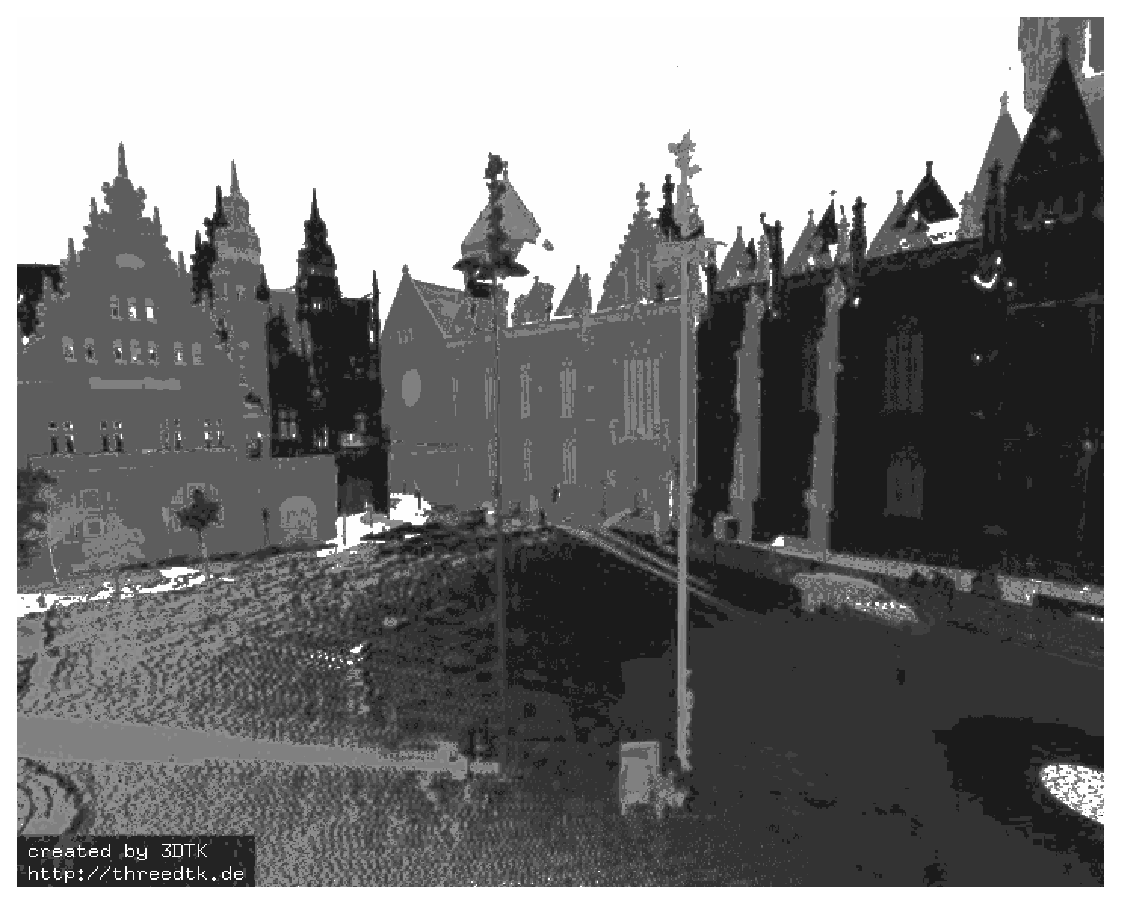
\includegraphics[width=0.75\linewidth]{BOOKFIGS/start_1}\\
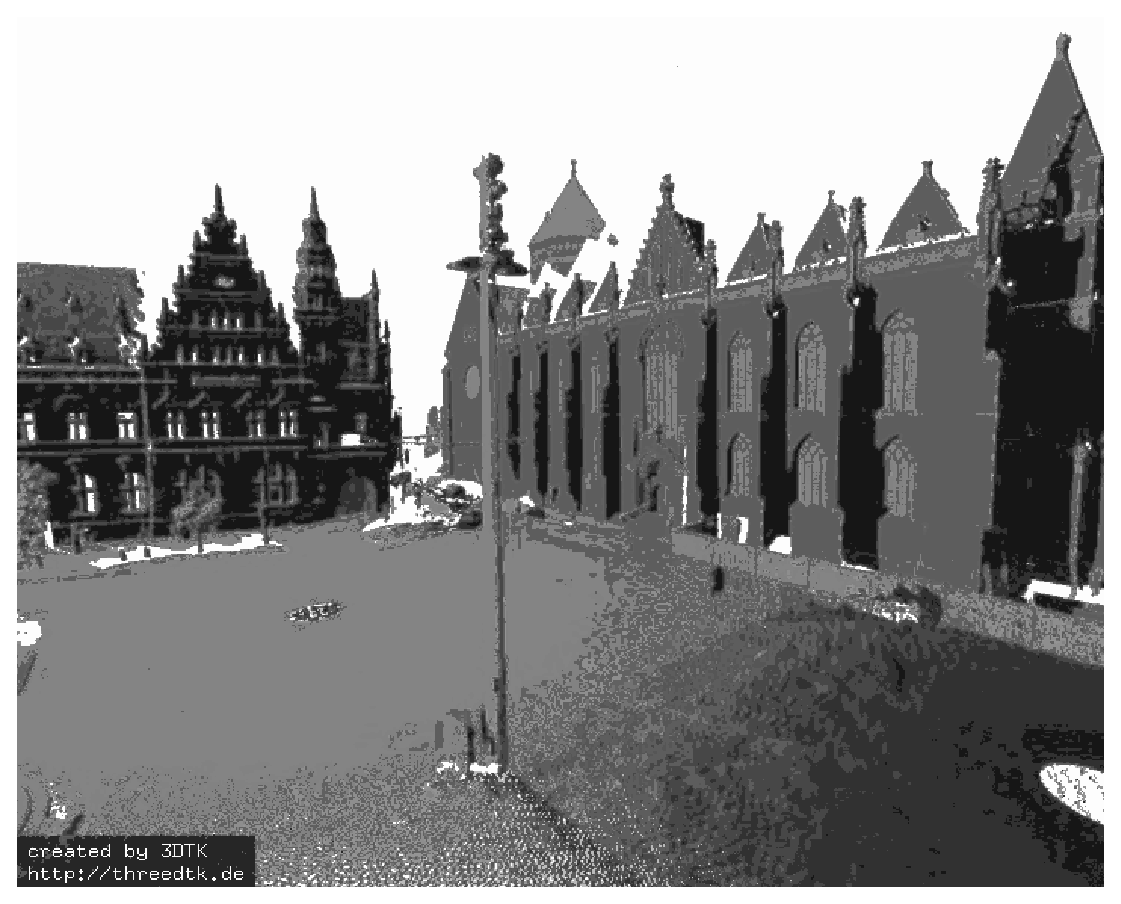
\includegraphics[width=0.75\linewidth]{BOOKFIGS/final_1}
\caption{Initial alignment of two 3D pint clouds (top) and after
  optimization with ICP (bottom).}\label{fig:icp}
\end{figure}  

Implementations of ICP (cf. algorithm~\ref{algo:ICP}) use a maximal
distance for closest points to handle partially overlapping point
sets. In this case, the proof about ICP's monotonic convergance
in~\cite{besl2} no longer holds, since the number of points as well as
the value of $E(\M R, \V t)$ might increase after applying a
transformation.

\begin{algorithm}
\caption{The ICP algorithm.}\label{algo:ICP}
\begin{algorithmic}[1]
\vspace*{2mm}
\FOR {$i = 0$ to \textit{maxIterations}}
  \FORALL {$\V d_j \in D$}
    \STATE {find the closest point within a range $d_\text{max}$ in the
      set $M$ for point $\V d_j$}
  \ENDFOR

  \STATE {Calculate transformation ($\M R, \V t$) that minimizes the
    error function Eq. (\ref{DMin})}

  \STATE  Apply the transformation found in step 5 to the data set
           $D$.

  \STATE Compute the difference of the quadratic error, i.e., compute the
  difference of the value $\norm{E_{i-1}(\M R, \V t) - E_i(\M R, \V t)}$
  before and after the application of the transformation. If this
  difference falls below a threshold
  $\varepsilon$, terminate.
\ENDFOR
\vspace*{2mm}
\end{algorithmic}
\end{algorithm}

Current research in the context of ICP algorithms mainly focuses on
fast variants of ICP algorithms~\cite{Rusi_2001}. If the input are 3D
meshes then a point-to-plane metric can be used instead of
Eq.~\eqref{DMin}. Minimizing using a point-to-plane metric outperforms
the standard point-to-point one, but requires the computation of
normals and meshes in a pre-processing step.

The computation of closest points is the crucial step of the ICP
algorithm. A naive implementation examines all points in $\hat M$ and
the resulting computation time for ICP is $O(|\hat D|\,|\hat M|)$,
i.e., $O(n^2)$. Note: $\hat N$ can be very large; advanced
high-precise 3D laser scanners such as the Zoller+Fr\"ohlich yield a
data rate up to 1.000.000 3D points per second. An efficient tree data
structure, a $k$-d tree, is widely used to speed-up the closest point
computation. Every node of the $k$-d tree represents a partition of
the point set into two distinct sets, the successor nodes. The root of
the tree represents the whole point set. The leaves of the tree are
called buckets and are a partition of the set into small, disjunctive
point sets. Furthermore, every node of the tree consists of the center
and the dimension of the point set.  In the original $k$-d tree paper,
these so-called split dimensions have been chosen depending of the
depth of node in a robin-round fashion~\cite{Bentley_1975}.  The split
dimension and value define an axis-aligned hyperplane in the
$k$-dimensional space. The data are partitioned according to their
position to the hyperplane into the successor nodes. The $k$-d tree is
constructed until the number of points in the nodes falls below a
threshold $b$ (bucket size). Only the leaves of the tree contain the
data points. Searching in $k$-d trees is done recursively. A given 3D
point $\V p_q$ needs to be compared to the separating plane (splitting
dimension and splitting value) in order to decide on which side the
search must continue. This procedure is executed until the leaves are
reached. There, the algorithm has to evaluate all bucket
points. However, the closest point may be in a different bucket, iff
the distance $d$ of the query point $\V p_q$ to the limits is smaller
than the one to the closest point in the bucket $\V p_b$.  In this
case backtracking has to be performed. The test is known as
Ball-Within-Bounds test~\cite{Bentley_1975, Friedman_1977,
  Greenspan_2003}. The optimized $k$-d tree choses the split dimension
and split value~\cite{Friedman_1977}, such that the expected amount of
backtracking is minimized.  Since one typically has no information
about the query points $k$-d tree algorithms take only the
distribution of the given points into account. For all possible
queries this works sufficiently, but it will not be optimal for a
specific query~\cite{Friedman_1977}. This enables the recursive
construction and avoids the overall optimization that is known to be
NP-complete~\cite{Hyafil_1977}.

Improvements to $k$-d tree search, especially for small dimensions,
have been presented in the last decade. They include approximate $k$-d
tree search~\cite{Greenspan_2003}, registration using
$d$2-trees~\cite{Mitra_2004} and cached $k$-d tree search
\cite{3DIM_2007}. In addition, the spatial data structure oc-tree
might, which is discussed later in this section, can used to search
the point clouds with similar performance.

In each ICP iteration, the transformation can be calculated in $O(N)$
by any of these four methods: (1) a singular value decomposition (SVD)
based method by Arun et al.~\cite{arun}, (2) a quaternion based
method by Horn~\cite{Horn_1988}, (3) an algorithm using orthonormal
matrices by Horn et al.~\cite{Horn_1987}, and (4) a calculation based
on dual quaternions by Walker et al.~\cite{Walker_1991}. Besides these
closed-form solutions, there are several linearized, approximative
version~\cite{CVIU2010}. The challenge is to ensure thar $\M R$ is
orthonormal. Most often, the first method is implemented, due to it's
simplicity and the availability of numerical SVDs in various
libraries. The rotation $\M R$ is represented as an orthonormal $3
\times 3$ matrix.  The optimal rotation is calculated by $\M R = \M V
\M U^T$. Here the matrices $\M V$ and $\M U$ are derived by the SVD
$\M H = \M U \M \Lambda \M V^T$ of a cross correlation matrix $\M
H$. This $3 \times 3$ matrix $\M H$ is given by
\begin{align}
\M H =  \sum_{i=1}^{N} \V m'^T_i \V d'_i 
 =  \begin{pmatrix}
S_{xx} & S_{xy} & S_{xz} \\
S_{yx} & S_{yy} & S_{yz} \\
S_{zx} & S_{zy} & S_{zz} \\
\end{pmatrix}, \label{korrelation} 
\end{align}
where $S_{xx} = \sum_{i=1}^{N} \ m'_{x,i} d'_{x,i}, \ S_{xy} =
\sum_{i=1}^{N} \ m'_{x,i} d'_{y,i}, \ \ldots \, $.

\subsection{Marker and Feature-based Registration} 

To avoid issues with starting guess in the ICP framework, marker based
registration uses defined artificial or natural landmarks as
corresponding points. This manual data association ensures that by
minimizing Eq.~\eqref{DMin} the scans are registered at the correct
location. Iterations are no longer required, but possible a
verification with the RANSAC algorithm. The RANSAC algorithm is a
general, randomized procedure that iteratively finds an accurate model
for observed data that may contain a large number of
outliers~\cite{ransac}.

\subsubsection{3D Feature Representations and Extraction}\label{3d_feature_extraction.ch31}

There are many representations available for encoding 3D scene
structure and model representations, but the following representations
are the ones most commonly encountered in robotics applications. Some
scene models or descriptions may use more than one of these
simultaneously to describe different aspects of the scene or object
models.

\begin{itemize}

\item {\bf Normals \index{Normal}}:

  Normals describe the surface orientation in a points. There are a
  number of approaches that have been developed for computing normals
  in point clouds and range images. Most of these approaches involves
  some form of eigenvalue decomposition resembling total linear least
  squares. The normals are usually computed when taking into account
  the nearby neighbor points which are computed using a variety of
  meth- ods like Nearest Neighbor Search. These methods include $k$
  Nearest Neighbors ($k$NN) and radius search among others. The method
  of total least squares is robust to noise as it inherently includes
  low pass filtering but it sensitive to the distribution and density
  of the point samples as well as the curvature of the underlying
  manifold. Improvements to the above method by using higher order
  surfaces are discussed in~\cite{Mitra_2003} and it is noted that
  such methods can fail even with arbitrarily dense samples.

  The total least squares problem is finding the plane parameters
  that optimally fit a small surface area in a point set given by the 
  the nearest neighbors. A plane is defined by the equation
\begin{align*}
  n_x x + n_y y + n_z z - d = 0
\end{align*}  
  where $\V p = (x, y, z)^T$ lies on the plane and $(n_x, n_y, n_z,
  d)$ are the parameters to compute. Given a subset of $k$ 3D points
  $p_i, i = 1, 2, \ldots, k$ of the surface, least squares finds the
  optimal normal vector $n = (n_x, n_y, n_z )^T$ and scalar $d$ that
  minimizes the following error equation
\begin{align}
  e = \sum_{i=1}^k (\V p_i \V n - d)\label{eq:normal}
\end{align}  
  The basic method for normal estimation from the neighboring points
  using a fitting a plane is the Principal Component Analysis (PCA).
  PCA is the eigenvalue decomposition of the data covariance (or
  correlation) matrix or singular value decomposition of a data
  matrix, usually after mean centering (and normalizing) the data
  matrix for each attribute (3D query point). PCA can be interpreted
  as fiting a Gaussian distribution and computing the main axes. For
  each query point
\begin{align*}
  \V \mu    & = \frac{1}{k} \sum_{i=1}^{k} \V p_i \\
  \M \Sigma & = \frac{1}{k} \sum_{i=1}^{k} (\V p_i - \V \mu)^T(\V p_i - \V \mu)
\end{align*}
  The vector corresponding to the smallest eigenvalue of the above
  matrix $\M \Sigma$ is the normal direction if the neighboring
  points belong to a plane and this is also the closed form
  solution of the total least squares problem.

  For equirectangular range images, i.e., spherical coordinates, a
  fast algorithm has been developed in~\cite{Badino_2011} that avoids
  computing eigenvalues. Dividing \eqref{eq:normal} by $d^2$ gives a
  simplified function and further division by the squared range
  $\rho^2$ yields
\begin{align*}
  e = \sum_{i=1}^k \left( (\rho^{-1}\V p_i)^T \V n - \rho_i^{-1}\right)^2
  \qquad
  \V p_i =
  \begin{pmatrix}
    \cos \theta_i \sin \phi_i\\
    \sin \theta_i \sin \phi_i\\
    \cos \phi_i
  \end{pmatrix}
\end{align*}  
  Therefore, a solution for $\V n$ is given as:
\begin{align*}
  \V n = \M M^{-1} \V b \quad \text{where} \ \M M = \sum_{i=1}^{k}\V p_i \V p_i^T,
  \V b = \sum_{i=1}^{k} \frac{\V p_i}{\rho_i}.
\end{align*}
  This way the computation of eigenvalues is avoided and the matrix
  $\M M$ can be precomputed for the desired image coordinates as it
  does not depend on the range. The tangential surface and therefore
  its normal vector is obtained by simply taking the derivative of
  the surface function in the point of interest.
\begin{align*}
  \V n
  & = \nabla \rho = \nabla \rho(\theta,\phi)\\
  & = \begin{pmatrix}
    \cos \theta \sin \theta
    - \frac{\sin \theta}{\rho \sin \phi} \frac{\partial \rho}{\partial \theta}
    + \frac{\cos \theta \cos \phi}{\rho} \frac{\partial \rho}{\partial \phi}\\
    \sin \theta \sin \theta
    - \frac{\cos \theta}{\rho \sin \phi} \frac{\partial \rho}{\partial \theta}
    + \frac{\sin \theta \cos \phi}{\rho} \frac{\partial \rho}{\partial \phi}\\
    \cos \phi - \frac{\sin \phi}{\rho} \frac{\partial \rho}{\partial \phi}
    \end{pmatrix}
\end{align*}

  
\item {\bf 3D Point Features \index{Point Features}}:

  This is a set $\{ \V p_i = (x_i,y_i,z_i)\}$ of 3D points that
  describe some salient and identifiable points in the scene. They
  might be the centers of spheres (often used as markers), corners
  where 3 planes intersect, or the extrema of some protrusion or
  indentation on a surface.  They may be a subset of an initially
  acquired 3D full scene point set, or they might be extracted from a
  range image, or they might be computed theoretical points based on
  extracted data features.

  An early example of 3D Point features and descriptors are Spin Images,
  which are used for surface matching between point clouds and meshes.
  Scanned 3-D points become the vertices of the mesh and connectivity
  is established by the 3-D scanning geometry. A fundamental component
  of the surface matching representation is an oriented point, a
  three-dimensional point with an associated direction.  Huber et
  al. define an oriented point $\V O$ at a surface mesh vertex using
  the 3-D position of the vertex $\V p$ and the surface normal at the
  vertex $\V n$~\cite{HuberPhD}.  Two coordinates can be calculated
  given an oriented point: $\alpha$ the radial distance to the surface
  normal line $L$ and $\beta$ the axial distance above the tangent
  plane $P$ (cf.~Figure~\ref{fig:spinimage}).
  \begin{align*}
    \begin{array}{l}
  (\V x) \mapsto (\alpha, \beta) = \\[1.1ex]
    (\sqrt{||\V x - \V p||^2 - ( \V n \cdot (\V x -\V p))^2},
      \V n \cdot (\V x - \V p))
      \end{array}
  \end{align*}
  \begin{figure}
    \centering
    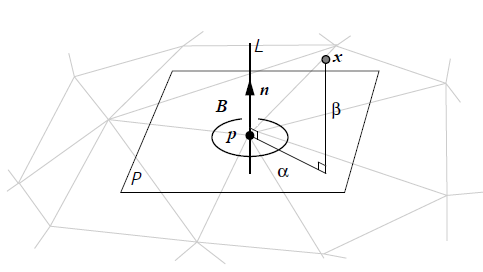
\includegraphics[width=0.75\linewidth]{BOOKFIGS/spinimage}
    \caption{Definition of a spin image.}\label{fig:spinimage}
  \end{figure}

  The term spin-map originates from the cylindrical symmetry of the
  oriented point basis; the basis can spin about its axis with no
  effect on the coordinates of points with respect to the
  basis~\cite{HuberPhD}. A consequence of the cylindrical symmetry is
  that points that lie on a circle that is parallel to $P$ and centered
  on $L$ will have the same coordinates $(\alpha,\beta)$ with respect
  to the basis.
 
  Seminal work on 3D point features are the Point Feature Histograms
  (PFH) descriptors. They encode a point's $k$-neighborhood geometrical
  properties by generalizing the mean curvature around the point using
  a multi-dimensional histogram of values~\cite{RaduPhD}. This highly
  dimensional hyperspace aims at providing an informative signature
  for the feature representation, aims at being invariant to the 6D
  pose of the underlying surface, and aims at coping very well with
  different sampling densities or noise levels present in the
  neighborhood~\cite{pointclouds.org}.

  To formulate the new feature space, the concept of a dual-ring
  neighborhood is first introduced.  Following the notation and the
  text of~\cite{RaduPhD} let $P$ be a set of 3D points with $x_i, y_i,
  z_i$ the geometric coordinates. A point $\V p_i$ of $P$ is said to
  have a dual-ring neighborhood if:
  \begin{align*}
  r_1, r_2 \in R \ r_1 < r_2 \
  \text{, such that}
  \left\{
  \begin{array}{l}
    r_1 \to P^{k_1}\\
    r_2 \to P^{k_2}
  \end{array}
  \right.
  \end{align*}
  with $0 < k_1 < k_2$. The two radii $r_1$ and $r_2$ are used to
  determine two distinct layers of feature representations for $\V
  p_i$. The first layer represents the surface normal at the query
  point from the neighborhood patch $P^{k_1}$. The second layer
  comprises the Point Feature Histogram as a set of angular features
  (cf. Fig.~\ref{fig:angular_feature}):
  \begin{align*}
    \alpha & = \V v \cdot \V n_t \\
    \phi   & = \V u \cdot \frac{(\V p_t - \V p_s)}{d}\\
    \theta & = \arctan(\V w \cdot \V n_t, \V u \cdot \V n_t)
  \end{align*}
  \begin{figure}
    \centering
    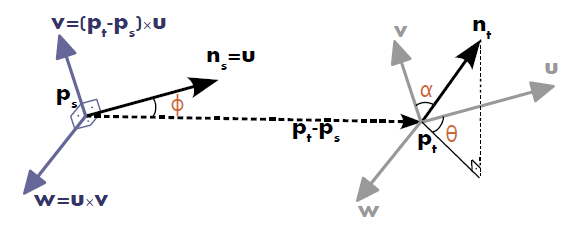
\includegraphics[width=0.85\linewidth]{BOOKFIGS/angular_feature}
    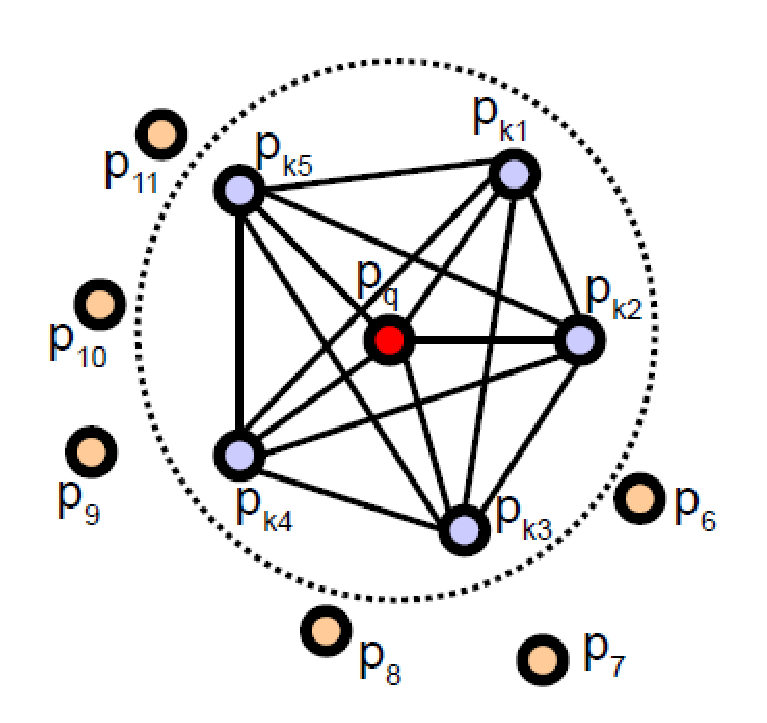
\includegraphics[width=0.6\linewidth]{BOOKFIGS/pfh}
    \caption{Angular features in PFHs (top) and the definition of the
      two regions (bottom).}\label{fig:angular_feature}
  \end{figure}  

  In addition to 3D structural features, 3D features derived from
  texture, e.g., co-registered color images or scan reflectivities,
  are widely used for registration~\cite{Boehm_2007,rgbdslam}.
  Fig.~\ref{fig:scansift} shows SIFT features extracted from a 3D
  scanner with calibrated reflectivity values.
  \begin{figure}
    \centering
    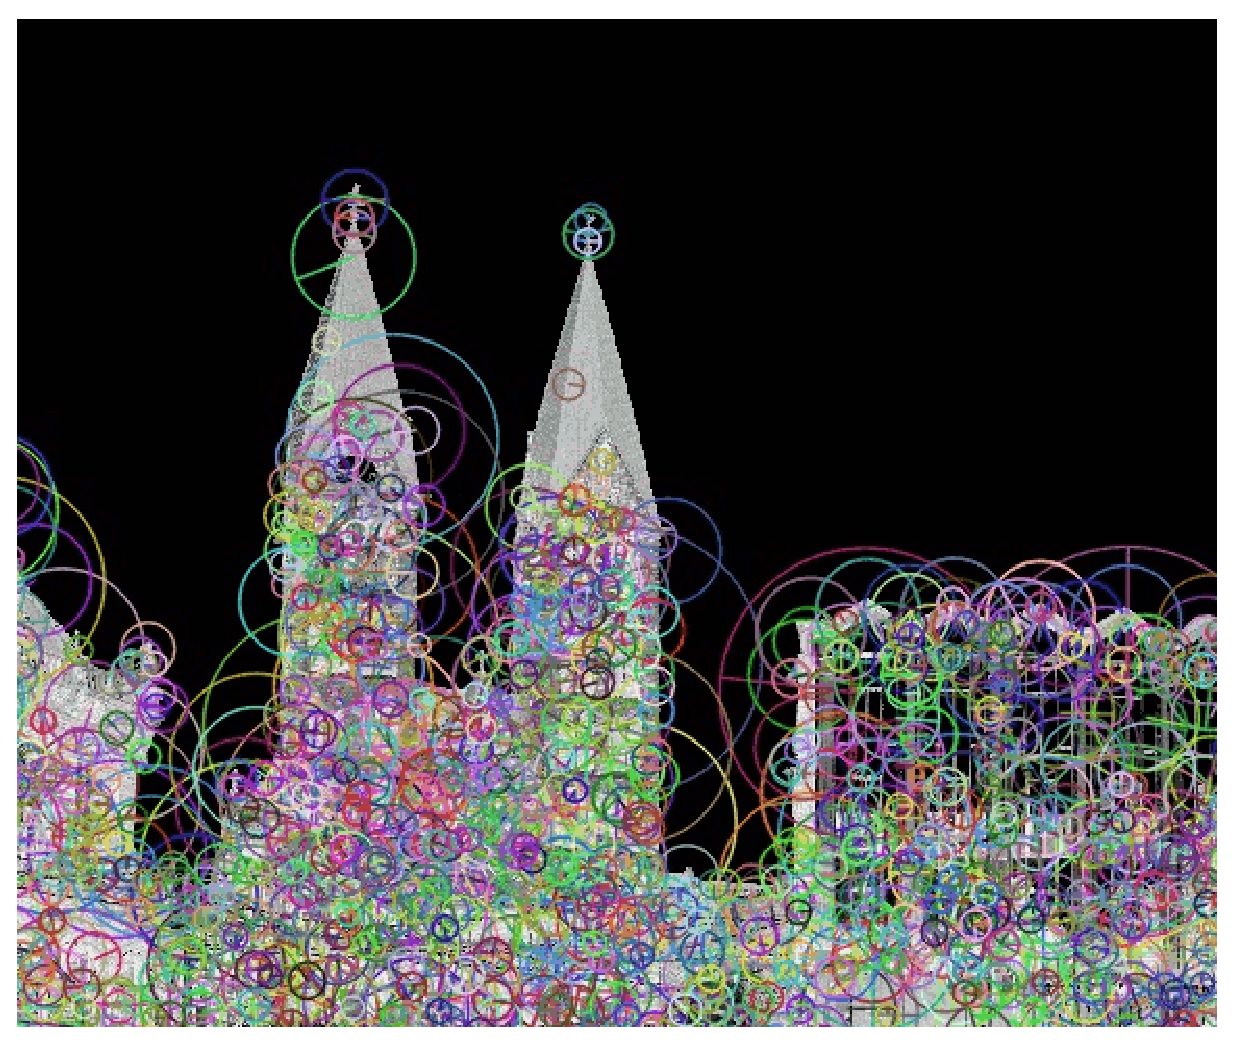
\includegraphics[width=0.8\linewidth]{BOOKFIGS/scansift}
    \caption{Sift features extracted from the reflectivity values of a
      3D laser scan.}\label{fig:scansift}
  \end{figure}  
  
\item {\bf Planes}:
  
  A planar surface may only be described by the infinite surface as
  given by the equation, but it may also include a description of the
  boundary of the surface patch. Convenient representations for
  robotics applications are lists of the 3D points $\{(x_i,y_i,z_i)\}$
  that form the patch boundary, or polylines, which represent the
  boundary by a set of connected line segments. A polyline is
  represented by the sequence of 3D points $\{(x_i,y_i,z_i)\}$ that
  form the vertices that join the line segments.

  Plane extraction, or plane fitting, is the problem of modeling a
  given 3D point cloud as a set of planes that ideally explain every
  data point. The RANSAC algorithm is one possible algorithm. When
  adapted for plane finding, this algorithm selects three 3D points at
  random (although exploiting some locality to the point selection
  algorithm can improve the efficiency of the algorithm). These three
  points determine a plane with parameter vector ${\bf \it a}$.  Test
  all points $\{ \V p \}$ in the set for belonging to the plane
  ({\it i.e.} $\mid \V p_i \cdot \V a \mid < \tau$).  If
  enough points are close to the plane, then potentially a plane has
  been found.  These points should also be processed to find a
  connected set, from which a more accurate set of plane parameters
  can be estimated using the least-square algorithm given above.  If a
  planar patch is successfully found, the points that lie in that
  plane are removed from the dataset.  The random selection of three
  points then continues until no more planes are found (a bound on how
  many tries to make can be estimated). For example Schnabel et
  al.~\cite{Schnabel:2007} have adapted RANSAC for plane extraction
  and found that the algorithm performs precise and fast plane
  extraction, but only if the parameters have been fine-tuned
  properly. For their optimization they use knowledge, that is not
  readily available in point cloud data, such as normals, neighboring
  relations and outlier ratios.

  A further standard method for plane detection is region growing,
  based on a seed patch. When the scene largely consists of planes, a
  particularly simple approach is based on selecting a previously
  unused point and the set of points $\{\V p_i = (x_i,y_i,z_i)\}$ in
  its neighborhood. A plane is fit to these points using the least
  square method (cf. normal computation).  This hypothesized plane
  then needs to be tested for reasonableness by 1) examining the
  smallest eigenvalue - it should be small and on the order of the
  square of the expected noise level and 2) ensuring that most of the
  3D points in the fitted set lie on the plane ({\it i.e.} $\mid
  {\V p}_i \cdot \V a \mid < \tau$).

  Larger planar regions are ``grown'' by locating new adjacent points
  $\V p_i$ that lie on the plane ({\it i.e.} $\mid \V p_i \cdot \V a
  \mid < \tau$).  When enough of these are found, the parameters $\V
  a$ of the plane are re-estimated.  Points on the detected plane
  are removed and the process is repeated with a new seed patch.
  This process continues until no more points can be added.
  complete descriptions of planar feature extraction with region
  growing is given in~\cite{hoover}.

  Bauer et al. use the radon transform to detect planes in volume
  data~\cite{Bauer:2008}. The idea and the speed of the algorithm are
  similar to that of the Standard Hough Transform. The Hough
  Transform~\cite{Hough:1962} is a method for detecting parametrized
  objects. For the Hough transform planes are represented in the Hesse
  normal form, using normal vectors. A plane is thereby given by a
  point $\V{p}$ on the plane, the normal vector $\V{n}$ that is
  perpendicular to the plane and the distance $\rho$ to the origin
  \begin{align*}
    \rho = \V p \cdot \V n  = {p}_x {n}_x + {p}_y {n}_y + {p}_z {n}_z = \rho .
  \end{align*}
  Considering the angles between the normal vector and the coordinate
  system, the coordinates of $\V n$ are factorized to
  \begin{align}
    {p}_x \cdot \cos{\theta} \cdot \sin{\varphi} + {p}_y \cdot \sin{\varphi} \cdot \sin{\theta} + {p}_z \cdot \cos{\varphi} = \rho ,
    \label{eq:polar}
  \end{align}
  with $\theta$ the angle of the normal vector on the $xy$-plane and
  $\varphi$ the angle between the $xy$-plane and the normal vector in
  $z$ direction. $\varphi$, $\theta$ and $\rho$ define the
  3-dimensional Hough Space ($\theta,\varphi,\rho$) such that each
  point in the Hough Space corresponds to \emph{one plane} in
  $\mathbb{R}^3$. To find planes in a point set, one calculates the
  Hough Transform for each point. Given a point $\V p$ in Cartesian
  coordinates, one finds all planes the point lies on, i.e., find all
  the $\theta$, $\phi$ and $\rho$ that satisfy Eq.~\eqref{eq:polar}
  Marking these points in the Hough Space, i.e., leads to a 3D
  sinusoid curve as shown in Fig.~\ref{fig:houghcurve}. The
  intersections of two curves in Hough Space denote the planes that
  are rotated around the line built by the two points. Consequently,
  the intersection of three curves in Hough Space corresponds to the
  polar coordinates defining the plane spanned by the three points. In
  Fig.~\ref{fig:houghcurve} the intersection is marked in black.
  %
  Given a set $P$ of points in Cartesian coordinates, one transforms
  all points $\V{p}_i \in P$ into Hough Space. The more curves
  intersect in $\V{h}_j \in (\theta, \varphi, \rho)$, the more points
  lie on the plane represented by $\V{h}_j$ and the higher is the
  probability that $\V{h}_j$ is actually extracted from $P$.
  %
  \begin{figure}
    %\psfrag{phi}{$\varphi$}
    %\psfrag{theta}{$\theta$}
    %
    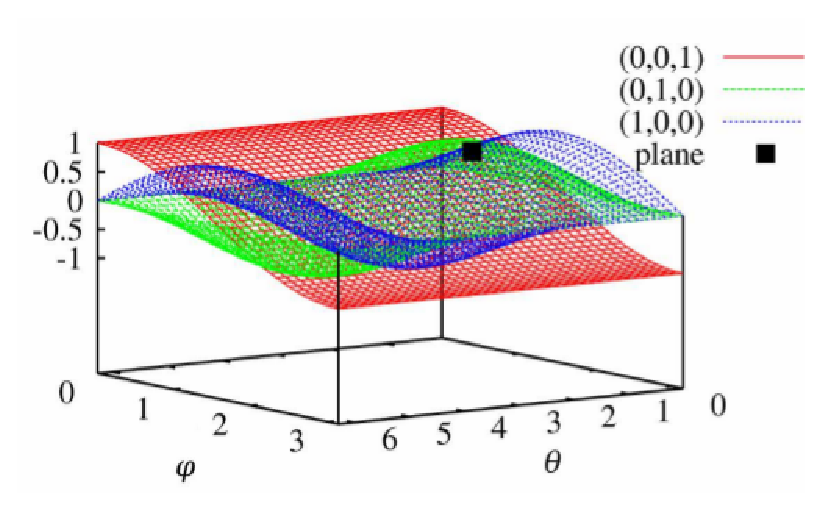
\includegraphics[width=0.4\textwidth]{BOOKFIGS/Hough}
    \caption{Transformation of three points from $R$ to % FIXME mathbbm R
      Hough space ($\theta,\varphi,\rho$). The intersection of the
      curves (marked in black) depicts the plane spanned by the three
      points.}
    \label{fig:houghcurve}
  \end{figure}
  %  

  The Standard Hough Transform is far too slow for plane detection in
  real world data. A variant called Randomized Hough Transform is the
  method of choice when dealing with 3D data due to its exceptional
  performance as far as runtime and quality is
  concerned~\cite{Borrmann_2011}.
  
  Other plane extraction algorithms are highly
  specialized for a specific application and are not in widespread use
  for miscellaneous reasons. Lakaemper et al.~\cite{Lakaemper:2006}
  use an Expectation Maximization (EM) algorithm to fit planes that
  are initially randomly generated, Wulf et al.~\cite{Wulf:2004}
  detect planes relying on the specific properties of a sweeping laser
  scanner and Yu et al.~\cite{Yu:2008} developed a clustering approach
  to solve the problem.  

\item {\bf Triangulated Surfaces \index{Triangulated Surfaces}}:

  Most commonly, surfaces are approximated by polygonal meshes,
  particularly triangle meshes, a standard data structure in computer
  graphics to represent 3D objects. This representation describes an
  object or scene by a set of triangular patches. More general
  polygonal surface patches or even various smooth surface
  representations are also used, but triangles are most commonly used
  because they are simpler and there are inexpensive PC graphics cards
  that display triangles at high speed.

  The triangles can be large ({\it e.g.} when representing planar
  surfaces) or small ({\it e.g.} when representing curved surfaces).
  The size chosen for the triangles reflects the accuracy desired for
  representing the object or scene surfaces.  The triangulated surface
  might be complete in the sense that all observable scene or objects
  surfaces are represented by triangles, or there might be
  disconnected surface patches with or without internal holes.  For
  grasping or navigation, you don't want any unrepresented scene
  surface to lie in front of the represented portion of the surface
  where a gripper or vehicle might collide with it.  Hence, we assume
  that the triangulation algorithms produce patch sets that, if
  completely connected at the edges, implicitly bound all real scene
  surfaces. Figure~\ref{timmesh} shows an example of a triangulated
  surface and the original point cloud.
\begin{figure}
    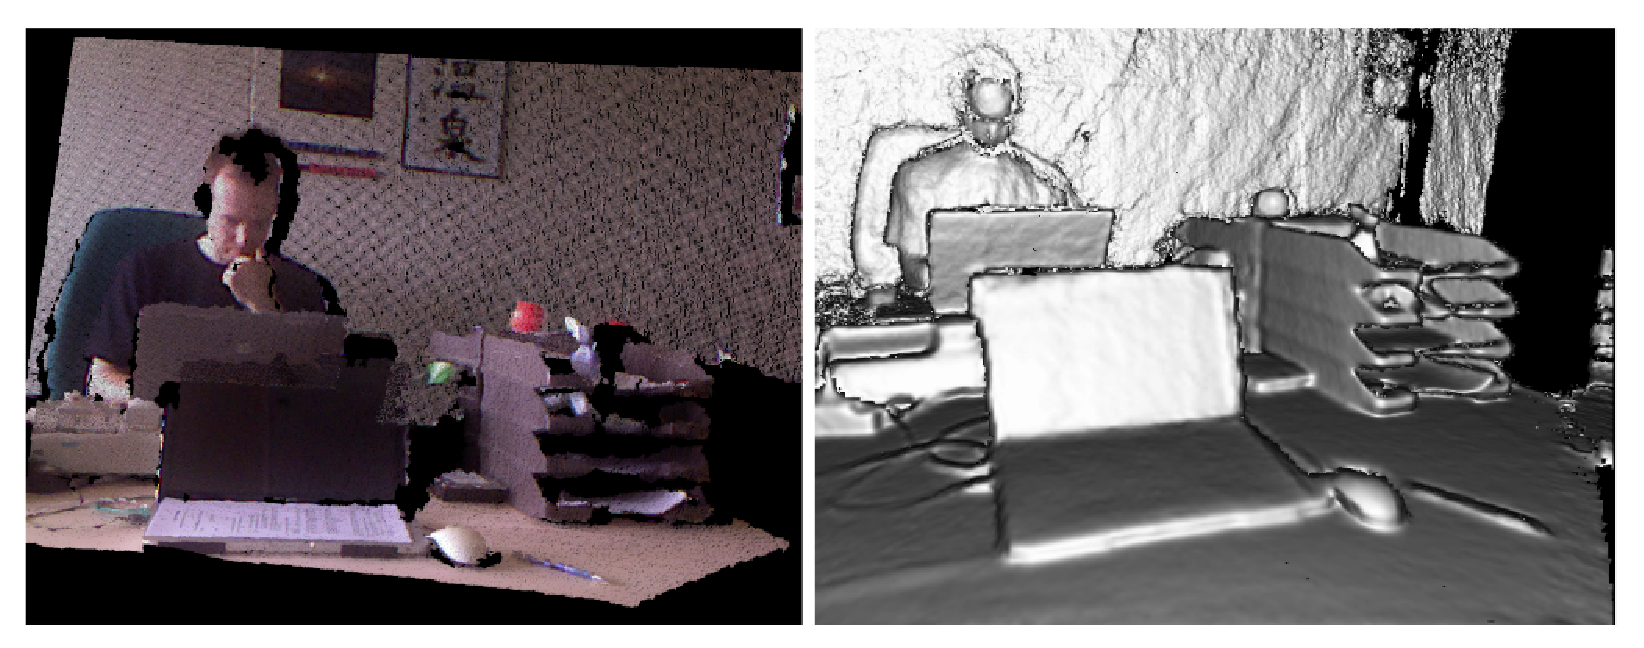
\includegraphics[width=0.5\textwidth]{BOOKFIGS/kinect_fusion}
\caption{Left: image acquired with a kinect-like sensor.
  Right: Reconstruction with kinect fusion. \label{timmesh}}
\end{figure}

  The de-facto standard is the Marching Cubes method introduced by
  Lorensen et al. \cite{lorensen87marching}. This algorithm
  sub-divides the scanned volume into cubic cells or voxels. For each
  cell the intersections between the cell edges and the surface are
  calculated. Pre-calculated surface patterns are then used to
  generate a local triangle mesh approximation. An example of such
  patterns are given in Fig.~\ref{fig:patterns}. To interpolate the
  intersections, implicit continuous surface representations like
  planes or splines are fitted to the local data using least squares
  fits~\cite{alexa02computing,hoppe}.
  %
  % FIXME More about Hoopes distance function
  %
  A feature of the Marching Cubes algorithm is that it produces more
  triangles than are needed to represent an object.  Hence, several
  mesh simplification algorithms have been introduced over the past
  years. Most of them define error metrics that indicate the error
  that a certain operation causes to the model, i.e., the removal of
  an edge~\cite{melax98simple, garland97surface}. To optimize the
  model, the edges causing minimal error to the topology are removed
  iteratively. Since after each edge removal new vertices have to be
  inserted into the mesh, the initial topology can be altered.
\begin{figure}
    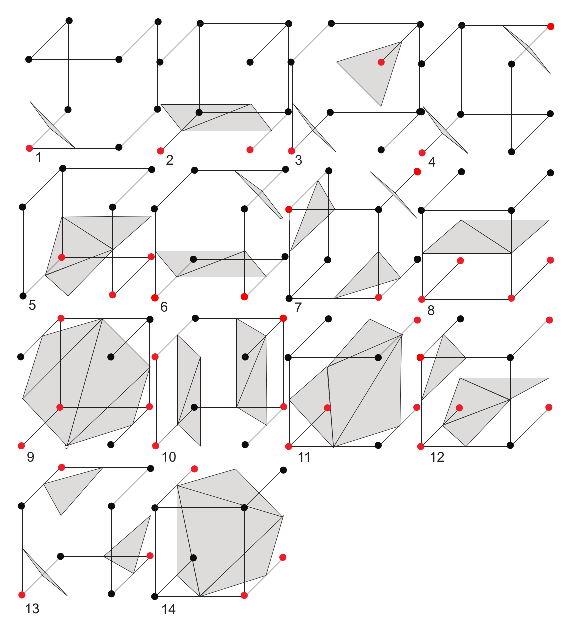
\includegraphics[width=0.5\textwidth]{BOOKFIGS/mc_cases_corrected}
\caption{Pattern for meshing 3D voxels. 256 combinations are possible,
  but it is sufficient to model 16, iff symmetries are considered.
\label{fig:patterns}}
\end{figure}

  The kinect fusion approach modifies Hoppe's distance
  function~\cite{kinectfusion}. It exploits the properties of the
  depth image (rectangular) to calculate normals and the associated
  planes. The method is massively parallelized by a GPU implementation
  and can reconstruct and register meshes in real-time.

\item {\bf 3D lines}:
  
  The 3D lines where planar surfaces meet are features that can be
  easily detected by both stereo and range sensors.  These features
  occur commonly in built environments ({\it e.g.} where walls,
  floors, ceilings and doorways meet, around the edges of wall
  structures like notice boards, at the edges of office and warehouse
  furniture, etc.).  They are also common on manmade objects.  In the
  case of stereo, changes of surface shape or coloring are detected as
  edges, which can be matched in the stereo process to directly
  produce the 3D edge.  In the case of a range sensor, planar surfaces
  can be easily extracted from the range data (see next section) and
  adjacent planar surfaces can be intersected to give the edges.

  The most straightforward representation for 3D lines is the set of
  points $\V x = \V p + \lambda \V v$ for all $\lambda$, where $\V v$
  is a unit vector.  This has 5 degrees of freedom; more complex
  representations {\it e.g.} with 4 degrees of freedom exist
  \cite{hartley}.

\item {\bf Voxels}

  The \index{voxel} voxel (volume pixel) approach represents the 3D
  world by 3D boxes/cells that indicate where there is scene structure
  and where there is free space.  The simplest representation is a 3D
  binary array, encoded as 1 for having structure and 0 for free
  space.  This can be quite memory intensive, and also requires a lot
  of computation to check many voxels for content.  A more complex but
  more compact representation is the hierarchical representation
  called the octree \cite{foley}. This divides the entire (bounded)
  rectangular space into 8 rectangular subspaces called octants (see
  Figure \ref{octree}).  A tree data structure encodes the content of
  each octant as empty, full or mixed.  Mixed octants are then
  subdivided into 8 smaller rectangular octants, encoded as subtrees
  of the larger tree.  Subdivision continues until some minimum octant
  size is reached.  Determining whether a voxel is empty, full or
  mixed depends on the sensor used, however, if no 3D data points are
  located in the volume of a voxel, then it is likely to be empty.
  Similarly, if many 3D points are present, then the voxel is likely
  to be full. Currently, many implementations using octrees for range
  data are available~\cite{ISPRS2013,Hornung_2013}. Furthermore, these
  voxel representations are the basis of surface/mesh reconstruction
  algorithms as describes earlier.
\begin{figure}
    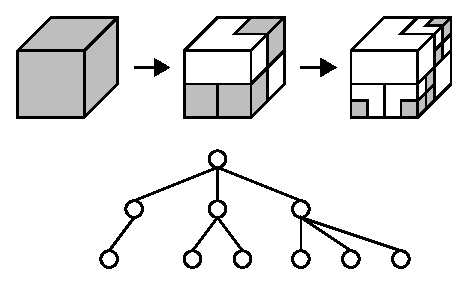
\includegraphics[width=0.4\textwidth]{BOOKFIGS/octree}
\caption{Top: Spatial subdivisions of an octree up to level
  3. Occupied leaf nodes are shaded grey.  Bottom: The corresponding
  tree structure of the sparse data structure. 
\label{octree}}
\end{figure}

  For the purpose of robot navigation, localization or grasping, only
  the surface and \index{free space voxels} free space voxels need to
  be marked accurately. The interior of objects and scene structure
  are largely irrelevant.

\item {\bf Straight lines}: 

  While straight lines are common in man-made scenes, direct
  extraction from 3D datasets is not easy.  The main source of the
  difficulty is 3D sensors often do not acquire good responses at
  edges of surfaces.
% -> Modern FWA scanners can do this!!!
% 1) the sensor beam will be sampling from two different surfaces and
% 2) laser based sensors produce somewhat unpredictable effects.
%
  For this reason, most 3D line detection algorithms are indirect,
  whereby planes are first detected, {\it e.g.} using the method of
  the previous section, and then adjacent planes are intersected.
  Adjacency can be tested by finding paths of connected pixels that
  lead from one plane to the other.
%
  If planes 1 and 2 contains points $\V p_1$ and $\V p_2$ and have
  surface normals $\V n_1$ and $\V n_2$ respectively, then the
  resulting intersection line has equation $\V x = \V a + \lambda \V
  d$ where $\V a$ is a point on the line and $\V d = \frac{\V n_1
    \times \V n_2} {\mid\mid \V n_1 \times \V n_2 \mid\mid}$ is the
  line direction.

  There are an infinite number of possible points $\V a$, which can be
  found by solving the equations $\V a' \V n_1 = \V p_1' \V n_1$ and
  $\V a' \V n_2 = \V p_2'\V n_2$. A reasonable third constraint that
  obtains a point near to $\V p_2$ is the equation $\V a' \V d = \V
  p_2' \V d$. This gives us an infinite line. Most practical
  applications require a finite segment. The endpoints can be
  estimated by 1) finding the points on the line that lie close to
  observed points in both planes and then 2) finding the two extremes
  of those points.  On the other hand, finding straight 3D lines can
  be easier with a stereo sensor, as these result from matching 2
  straight 2D image lines.

\end{itemize}

\subsection{Multiple-View Registration\label{match31}}\index{Multiple-View Registration}

A globally consistent representation of a robot's environment is
crucial for many robotic applications. Equipped with a 3D
depth-perceiving sensor, many mobile systems gather spatial
information about their local 3D environments. Any iterative
application of matching algorithms leads to inconsistencies due to
sensing errors and to the inaccuracies in the matching procedures
itself. To avoid these problems, global matching algorithms are
needed, taking global correspondences between range sensor data into
account. Simultaneous localization and mapping (SLAM) algorithms as
discussed in chapter \ref{FIXME} solve a very similar problem. In
addition to registering multiple views, they estimate a map.
Multiple-View Registration also relates to Bundle adjustment in the
photogrammetry community and structure from motion (SFM).

If $n$-views have to be registered, any sequential application of a
two point--set registration method will accumulate errors, and
therefore the registration algorithm (cf. section~\ref{sec:icp6D}) has
to be extended. The global error function becomes
\begin{align}
E & =  \sum_{l \to k} \sum_{i} \norm{(\M R_l \V m_{l,i} + \V t_l) - (\M R_k \V d_{k,i}
 + \V t_k)}^2, \label{DMinGlobal}
\end{align}
where all views have their unique pose $(\M R, \V t)$. After the point
pairs for all overlapping views $(l,k)$ have been found,
Eq.~\eqref{DMinGlobal} is minimized. Unfortunately, a closed-form
solution for minimizing Eq.~\eqref{DMinGlobal} is not know, but a
small angle approximation or the helix transform yield a system of
linear equations that can be solved by Choleskey
decomposition~\cite{CVIU2010}. In an ICP-like fashion after every
transformation new point pairs have to be found
(cf. algorithm~\ref{algo:gICP}).
%
\begin{algorithm}
\caption{The globally consistent ICP algorithm.}\label{algo:gICP}
\begin{algorithmic}[1]
\vspace*{2mm}
\FOR {$i = 0$ to \textit{maxIterations}}
   \STATE {find the closest point within a range $d_\text{max}$ of
      every pair of overlapping 3D point clouds $(l,k)$.}
 
  \STATE {Calculate $n$ transformations ($\M R, \V t$) simultaneously
    that minimize the error function Eq. (\ref{DMinGlobal})}

  \STATE  Apply the $n$ transformations found in step 4 to all data sets.

  \STATE Compute the difference of the quadratic error, i.e., compute
  the difference of the value $\norm{E_{i-1} - E_i}$ before and after
  the application of the transformation. If this difference falls
  below a threshold $\varepsilon$, terminate.  \ENDFOR
\vspace*{2mm}
\end{algorithmic}
\end{algorithm}
%

A probabilistic SLAM-like notation of Eq.~\eqref{DMinGlobal} was
formulated in~\cite{lu97} for 2D range scans. For each pose ${\V X}$,
the term $\bar{\V X}$ denotes a pose estimate, and $\Delta {\V X}$ is
the pose error. The positional error of two poses ${\V X}_j$ and
${\V X}_k$ is described by:
\begin{align*}
E_{j,k} &= \sum^m_{i=1} \norm{ {\V X}_j \oplus {\V d}_i - {\V X}_k \oplus
{\V m}_i }^2 
\end{align*}
Here, $\oplus$ is the compounding operation that transforms a point
into the global coordinate system.  For small pose differences,
$E_{j,k}$ can be linearized by use of a Taylor expansion. With the
linearized error metric ${\V E}'_{j,k}$ and the Gaussian distribution
$(\bar{\V E}_{j,k}, {\M C}_{j,k})$ a Mahalanobis distance that
describes the global error of all the poses is constructed
\begin{align}
{\M W} &= \sum_{j \rightarrow k} (\bar{\V E}_{j,k} - {\V E}'_{j,k})^{T} {\M C}^{-1}_{j,k}
(\bar{\V E}'_{j,k} - {\V E}'_{j,k}) \nonumber \\
&=  \sum_{j \rightarrow k}
\bigl(\bar{\V E}_{j,k} - ({\V X}'_j - {\V X}'_k)\bigr)
{\M C}^{-1}_{j,k} \bigl(\bar{\V E}'_{j,k} - ({\V X}'_j - {\V X}'_k)\bigr),\label{eq:u1}
\end{align}
which can be solved efficiently using iterative least squares
techniques, e.g., Levenberg-Marquadt or conjugate gradient methods
\cite{konolige04,kelly03}.  The covariances are computed from point
pairs. In the presence of correct covariances, Eq.~\eqref{eq:u1} is
minimized once. In case of scan matching, new pose estimates yield new
closest point pairs and in turn new covariances. Iterating the process
of calculating point pairs and minimization yields a stable algorithm
that converges rapidly. The probabilisty notation and the global ICP
notation are very similar~\cite{CVIU2010}. The solution for 2D range
scans has been extended to to 6DoF in~\cite{RAS2007}.

\subsection{Model Matching}

Model matching is the process of matching some stored representation
to some observed data. In the case discussed here, we assume that both
are 3D representations.  Furthermore, we assume that the
representations being matched are both of the same type, {\it e.g.} 3D
model and scene lines. (While different types of data can also be
matched, we ignore these more specialized algorithms here.)

A special case of matching is when the two structures being matched
are both scene or model surfaces. The algorithm used for matching
depends on the complexity the structures being matched.  If the
structures being matched are extended geometric entities such as
planes or 3D lines, then a discrete matching algorithm like the
Interpretation Tree algorithm \cite{grimson} can be used. It is
suitable for matching small numbers ({\it e.g.} less than about 20-30)
discrete objects, such as vertical edges seen in 2D or 3D. If there
are $M$ model and $D$ data objects, then potentially there are $M^D$
different matches. The key to efficient matching is to identify
pairwise constraints that eliminate unsuitable matches. Constraints
between pairs of model features and pairs of data features also
greatly reduce the matching space. If the constraints eliminate enough
features, a polynomial time algorithm results.  The core of the
algorithm is defined as follows.  Let $\{m_i\}$ and $\{d_j\}$ be the
sets po model and data features to be matched, $u(m_i,d_j)$ is true if
$m_i$ and $d_j$ are compatible features, $b(m_i,m_j,d_k,d_l)$ is true
if the four model and data features are compatible and $T$ is the
minimum number of matched features before a successful match is
declared.  \verb+Pairs+ is the set of successfully matched features.
The function \verb+truesizeof+ counts the number of actual matches in
the set, disregarding matches with the wildcard * which matches
anything.
%!!! get algorithm on 1 page !!!
\begin{verbatim}
pairs=it(0,{})
if truesizeof(pairs) >= T, then success

function pairs=it(level,inpairs)
  if level >= T, then return inpairs
  if M-level+truesizeof(inpairs) < T
    then return {} % can never succeed
  for each d_i % loopD start
    if not u(m_level,d_i), then continue loopD
    for each (m_k,d_l) in inpairs
      if not b(m_level,m_k,d_i,d_l)
        then continue loopD
    endfor
    % have found a successful new pair to add
    pairs = it(level+1,
                 union(inpairs,(m_level,d_i)))
    if truesizeof(pairs) >= T, then return
  endfor % loopD end

  % no success, so try wildcard  
  it(level+1,union(inpairs,(m_level,*)))
\end{verbatim}

\subsection{Relative Pose Estimation\label{pose23}} \index{Pose Estimation}

Central to many tasks is the estimation of the coordinate system
relative position or pose transformation between two coordinate
systems.  For example, this might be the pose of a scanner mounted on
a mobile vehicle relative to scene landmarks.  Or, it might be the
relative pose of some scene features as observed in two views taken
from different positions.

We present here three algorithms that cover most instances of the pose
estimation process, which differ slightly based on the type of feature
being matched.

\ \\
\noindent
{\bf Point set relative pose estimation}

The ICP algorithm can be used relative pose estimation as well
(cf.~\ref{sec:icp6D}).

\ \\
\noindent
{\bf Straight line relative pose estimation}

If 3D lines are the features that are extracted, then the relative
pose transformation can be estimated as follows.  Assume $N$ paired
lines.  The first set of lines is described by direction vectors $\{\V
e_i\}$ and a point on each line $\{\V a_i\}$.  The second set of lines
is described by direction vectors $\{\V f_i\}$ and a point on each
line $\{\V b_i\}$.  In this algorithm, we assume that the direction
vectors on the matched segments always point the same direction ({\it
  i.e.} are not inverted). This can be achieved by exploiting some
scene constraints, or trying all combinations and eliminating
inconsistent solutions. The points $\V a_i$ and $\V b_i$ need not
correspond to the same point after alignment. The desired rotation
matrix $\M R$ minimizes $\sum_i \mid\mid \M R \V e_i - \V f_i
\mid\mid^2$.  Construct the $3 \times N$ matrices $\M E$ that consists
of the vectors $\{ \V e_i \}$ stacked up. Construct the $3 \times N$
matrices $\M F$ in a similar way from the vectors $\{ \V f_i \}$.
Compute the singular value decomposition svd($\M F \M E'$) =
$\M U' \M D \M V'$. Compute the rotation
matrix\footnotemark[1] $\M R = \M V \M U'$. The
translation estimate $\V t$ minimizes the sum of the square of
the distances $\lambda_i$ between the rotated points $\V a_i$
and corresponding line $(\V f_i, \V b_i)$.  Define matrix
$\M L = \sum_i (\M I - \V f_i \V f_i')'(\M I - \V f_i')$.
Define the vector $\V n = \sum_i (\M I -\V f_i \V f_i')' (\M I -
\V f_i \V f_i') (\M R \V a_i - \V b_i)$.  Then the translation is
$\V t = - \V L^{-1}\V n$.

\ \\
\noindent
{\bf Plane relative pose estimation}

Finally, if planes are the 3D features extracted for matching, then
the relative pose transformation can be estimated as follows.  Assume
$N$ paired planes.  The first set of planes is described by surface
normals $\{ \V e_i \}$ and a point on each plane $\{\V a_i\}$.  The
second set of planes is described by surface normals $\{ \V f_i\}$ and
a point on each plane $\{ \V b_i\}$.  Here we assume that the surface
normals always point outward from the surface. The points $\V a_i$ and
$\V b_i$ need not correspond to the same point after alignment.  The
desired rotation matrix $\M R$ minimizes $\sum_i \mid\mid \M R \V e_i
- \V f_i \mid\mid^2$. Construct the $3 \times N$ matrices $\M E$ that
consists of the vectors $\{ \V e_i \}$ stacked up.  Construct the $3
\times N$ matrices $\M F$ in a similar way from the vectors $\{ \V f_i
\}$. Compute the singular value decomposition svd($ \M F \M E'$) = $\M
U' \M D \M V'$~\cite{arun}. Compute the rotation
matrix\footnotemark[1] $\M R$ = $\M V \M U'$.  The translation
estimate ${\bf \it t}$ minimizes the sum of the square of the
distances $\lambda_i$ between the rotated point $\V a_i$ and the
corresponding plane $(\V f_i, \V b_i)$. Define matrix $\M L = \sum_i
\V f_i \V f_i'$.  Define the vector $\V n= \sum_i \V f_i \V f_i' (\M R
\V a_i - \V b_i)$. Then the translation is $\V t= - \M L^{-1}\V n$.

In all of the calculations described above, we assumed normally distributed
errors. For techniques to robustify these sorts of calculations, see
Zhang~\cite{zhang}.

\subsection{3D Applications \label{3dapp}}

This section links the techniques presented above to the robotics applications
of 3D localization of parts for
robot manipulation, self-localization of robot vehicles and
scene understanding for robot navigation.
The robotics tasks mentioned here are discussed in more detail
in other chapters in the series.
While this chapter focusses on robotics applications, there are
many other 3D sensing applications. An area of much current research is
that of acquiring 3D models, particularly for reverse engineering of
mechanical parts \cite{benko},
historical artifacts \cite{levoy},
buildings \cite{stamos} and
people for computer games and movies (see, {\it e.g.}, Cyberware's Whole Body X 3D Scanner).


The key tasks in robot manipulation are:
(1) identification of grasping points (see Chapters 27 and 28),
(2) identification of a collision free grasp (see Chapters 27 and 28),
(3) recognition of parts to be manipulated (see Chapter 23) and
(4) position estimation of parts for manipulation (see Chapters 23 and 42).

The key tasks in robot navigation and self-localization are:
(5) identification of a navigable groundplane (see Section \ref{ch31.3}),
(6) identification of a collision free path (see Chapter 35),
(7) identification of landmarks (see Chapter 36) and
(8) estimation of vehicle location (see Chapter 40).

The mobile and assembly robotics tasks link together rather
naturally.
Tasks 1 \& 5 have a connection, when we consider these tasks
in the context of unknown parts or paths. Part grasping requires
finding regions on a part that are graspable, which usually means locally
planar patches that are large enough that a gripper can make good contact
with them.
Similarly, navigation usually requires smooth ground regions that are
large enough for the vehicle - again locally planar patches.
Both tasks are commonly based on triangulated scene methods to
represent the data, from which connected regions of nearly coplanar
patches can be extracted.
The main difference between these two tasks is the groundplane
detection task is looking for a larger patch, that must be on the
``ground'' and upward facing.

Tasks 2 \& 6 require a method of representing empty space along the 
proposed trajectory of the gripper contacts or the vehicle.
The voxel representation is good for this task.

Tasks 3 \& 7 are model matching tasks and can use the methods of
Section \ref{match31} to match observed scene features to prestored
models of known parts or scene locations.
Commonly used features are large planar surfaces, 3D edges and 3D feature
points.

Tasks 4 \& 8 are pose estimation tasks and can use the methods of
Section \ref{pose23} to estimate the pose of the object 
relative to the sensor or vehicle ({\it i.e.} sensor) relative to the scene.
Again, commonly used features are large planar surfaces, 3D edges and 3D feature
points.


\section{Navigation and Terrain Classification  \label{ch31.3}}

One of the more compelling uses for range data is for navigation of
mobile robot vehicles.  Range data provides information about
obstacles and free space for the vehicle, in a direct geometric form.
Because of the realtime constraints of navigation, it is often
impractical to reconstruct a full 3D model of the terrain using the
techniques presented in this Chapter.  Instead, most systems use an
{\em elevation model}. \index{elevation model} An elevation model is a tesselated 2D
representation of space, where at each cell there is information about
the distribution of 3D points in the cell.  In its simplest
incarnation, the elevation map just contains the mean height of range
points above the nominal ground plane (Figure
\ref{elevation_map.ch31}).  This representation is sufficient for some
indoor and urban environments; more sophisticated versions that
determine a local plane, scatter of points in the cell, etc., are
useful for more complicated off-road driving.  Elevation maps marked
with obstacles have obvious utility for planning a collision-free path
for the vehicle.

\begin{figure}[hbt]
{\epsfxsize = 0.5\textwidth \epsfbox{BOOKFIGS/elevation_map.eps}}
\caption{Elevation map in urban terrain.  Each cell holds the height
of the terrain at that point.  More extensive features can also be
incorporated: slope, point variance, etc.
\label{elevation_map.ch31}}
\end{figure}


\subsection{Indoor Reconstruction}

SLAM algorithms (Chapter 37) using 2D laser rangefinders can
reconstruct floor plans with centimeter precision.  Some research has
extended this work to 3D reconstruction, using 2D lasers that are
swept along as the robot moves \cite{thrun00}.  The resultant point
cloud is typically registered using the pose of the robot as corrected
by the 2D SLAM algorithm, rather than any of the 3D registration
techniques covered in this chapter, because the laser is swept using
robot motion.

The raw points can be presented as a 3D image, or triangulated to give
a planar or mesh reconstruction of indoor surfaces. \index{indoor surfaces}
The latter is
especially compelling when camera images are texture-mapped onto the
surfaces, creating a realistic 3D model.  Figure
\ref{indoor_3d_map.ch31} shows some results from indoor mapping using
this technique (from \cite{thrun00}).  Smoothing of surface facets can
be used to recover planar surfaces \cite{liu01}.

\begin{figure}[hbt]
{\epsfxsize = 0.5\textwidth \epsfbox{BOOKFIGS/thrun-3d-indoor.eps}}
\caption{3D indoor map from a swept vertical plane LADAR.
Registration is from a horizontal LADAR using SLAM algorithms (from
\cite{thrun00}). 
\label{indoor_3d_map.ch31}}
\end{figure}



\subsection{Urban Navigation}

In urban navigation, the environment is structured, with roads,
buildings, sidewalks, and also moving objects - people and other
vehicles.  There are two main challenges: how to register laser scans
from a fast-moving vehicle for consistent mapping, and how to detect
moving objects using range scans (of course, other methods are also
used for detecting moving objects, e.g., appearance-based vision).

Outdoor vehicles can use precision GPS, inertial measurement units,
and wheel odometry to keep track of their position and orientation,
typically with an extended Kalman filter.  This method is good enough
to obviate the need for precise registration matching among scans, as
long as the motion model of the vehicle, and timing from the range
scanner, is used to place each scan reading in its proper position in
the world model.  This method also works in relatively easy off-road
terrain such as in the DARPA Grand Challenge
\cite{GrandChallenge}.  In all cases, the reduction of pose
estimation error is critical for good performance
\cite{thrun06}. 

Once scan readings are registered using the vehicle pose estimation,
they can be put into an elevation map, and obstacles detected using
the slope and vertical extent of the range readings in the cells of
the map.  A complication is that there may be multiple levels of
elevation in an urban setting, for example, an overpass would not be
an obstacle if it were high enough.  One proposal is to use multiple
elevation clusters within each cell; this technique is called a {\em
multi-level surface map \index{surface map}} (MLS, \cite{triebel06}).
Each cell in the map stores a set of surfaces represented by a mean
height and variance.  Figure \ref{elev_map.ch31} shows an MLS with a
cell size of $10 {\rm cm}^2$, with ground plane and obstacles marked.

\begin{figure}[hbt]
{\epsfxsize = 0.50\textwidth \epsfbox{BOOKFIGS/mls_map.eps}}
\caption{Elevation map of an urban scene, using 10cm x 10cm cells.
Obstacles in red, ground plane in green (from \cite{triebel06}).
\label{elev_map.ch31}}
\end{figure}

For dynamic objects, realtime stereo at 15 to 30 Hz can capture the
motion of the objects.  When the stereo rig is fixed, range background
subtraction isolates just the moving objects \cite{eveland98}.  When
the rig is on a moving vehicle, the problem is more difficult, since
the whole scene is moving with respect to the rig.  It can be solved
by estimating the motion of the rig with respect to the dominant rigid
background of the scene.  Let $R,t$ be the motion of the rig between
two frames, estimated by extracting features and matching them across
the two temporal frames, using the techniques of Chapter 37.
The homography $H(R,t)$ of Equation
\ref{homography.eq.ch31} provides a direct projection of the disparity
vectors $p_0 = [x_0,y_0,d_0,1]$ of the first frame to their
correspondences $H(R,t)p_0$ under $R,t$ in the second frame.  Using
the homography allows the points in the reference frame to be directly
projected onto the next frame, without translating to 3D points.
Figure \ref{ind_motion.ch31} shows the projected pixels under rigid
motion from a reference scene.  The difference between the projected
and actual pixels gives the independently moving objects (from
\cite{agrawal05}).

\begin{figure*}[ht!]
{\epsfxsize = 0.95\textwidth \epsfbox{BOOKFIGS/independent_motion.eps}}
\caption{Independent motion detection from a moving platform.
Reference image on left is forward-projected using the motion homography to
the center image; right image is difference with actual image.
\label{ind_motion.ch31}}
\end{figure*}


\subsection{Rough Terrain} \label{ch31.roughterrain}

Rough outdoor terrain presents to challenges:
\begin{itemize}
\item There may be no extensive ground plane to characterize
driveability and obstacles.
\item Vegetation that is pliable and driveable may appear as an
obstacle in range images.
\end{itemize}

Figure \ref{rough_terrain.ch31} shows a typical outdoor scene, with a
small (1 meter) robot driving through vegetation and rough ground
\cite{konolige06}.  Range data from stereo vision on the robot will
see the top of the vegetation and some ground points below.  The
elevation model can be extended to look at {\em point statistics}
within each cell, to capture the notion of a local ground plane and
penetrability related to vegetation.  In \cite{ollis06}, for
example, the set of proposed features includes:
\begin{itemize}
\item Major plane slope using a robust fit (Section
\ref{3d_feature_extraction.ch31}). 
\item Height difference of max and min heights.
\item Points above the major plane.
\item Density: ratio of points in the cell to rays that pass through
the cell.
\end{itemize}
The density feature is interesting (and expensive to compute), and
attempts to characterize vegetation such a grass or bushes, by looking
at whether range readings penetrate an elevation cell.  The idea of
using vegetation permeability to range readings has been discussed in
several other projects on off-road driving
\cite{manduchi03,lalonde05,kelly05}.  

\begin{figure}[hbt]
{\epsfxsize = 0.40\textwidth \epsfbox{BOOKFIGS/rough_terrain.eps}}
\caption{Rough terrain, no ground plane, driveable vegatation.
\label{rough_terrain.ch31}}
\end{figure}

Elevation map cells can be characterized as obstacles or driveable
through learning or hand-built classifiers.  Among the learning
techniques are neural nets \cite{ollis06} and Gaussian mixture
models with expectation-maximization learning \cite{vandapel06}.
The latter work also includes a lower level of interpretation,
classifying surfaces into planar patches (ground plane, solid
obstacles), linear features (telephone wires), and scattered features
(vegetation).  Figure \ref{point_classified.ch31} shows some results
from a laser-scanned outdoor scene.  Linear features such as telephone
wires and the telephone pole are accurately determined, as well as
vegetation with high penetrability.

\begin{figure}[hbt]
{\epsfxsize = 0.40\textwidth \epsfbox{BOOKFIGS/point_stats_classified.eps}}
\caption{Classification using point statistics, from
\cite{vandapel06}.  Red is planar surface, blue is thin linear
surface, green is scattered penetrable surface.
\label{point_classified.ch31}}
\end{figure}

Some additional problems occur in \index{rough-terrain navigation} rough-terrain navigation.  For
planar laser rangefinders that are swept over the terrain by vehicle
motion, the precision of vehicle pose estimation is important for
accurate reconstruction.  Attitude errors of less than $0.5^o$ can
cause false positives in obstacle detection, especially for sweeps far
ahead of the vehicle.  In \cite{thrun06}, this problem is solved by
looking at the time of each laser reading, and noting a correlation
between height errors and time difference in the readings.

Negative \index{obstacles} obstacles (ditches and cliffs) are difficult to detect with
range information, because the sensor may not see the bottom of the
obstacle.  This is especially true for vehicle-mounted sensors that
are not very high off the ground, and that are looking far ahead.
Negative obstacles can be infered when there is a gap in the ground
plane, and a plane slanted upwards at the back edge of the gap.  Such
artifacts can be efficiently found using column search on the
disparity image \cite{bellutta00}.

\section{Conclusions and Further Reading}

Range sensing is an active and expanding field of research in
robotics.  The presence of new types of devices - flash ladars,
multi-beam ladars, on-camera stereo processing - and the continuing
development of robust algorithms for object reconstruction,
localization and mapping has helped to bring applications out of the
laboratory and into the real world.  Indoor navigation with ladars is
already being exploited in commercial products (see, for example,
\cite{karto}).  As the basic capabilities become more robust,
researchers are looking to perform useful tasks, such as fetching
items or doing dishes \cite{STAIR}.

Another set of challenges are found in less benign
environments, such as urban and off-road driving (DARPA Grand
Challenge and Urban Challenge \cite{GrandChallenge}).  Stereo vision
and laser rangefinding also will play a role in helping to provide
autonomy for a new generation of more-capable robotic platforms that
rely on walking for locomotion \cite{cmu-humanoid}.  The challenges are
dealing with motion that is less smooth than wheeled platforms,
environments that contain dynamic obstacles, and task-oriented
recognition of objects.  




\bibliographystyle{latex8}
\begin{thebibliography}{99}

\bibitem{adan}
A. Adan, F. Molina, L. Morena, 
``Disordered patterns projection for 3D motion recovering'',
Proc. Int. Conf. on 
3D Data Processing, Visualization and Transmission, pp 262-269, Thessaloniki, 2004.

\bibitem{agrawal05}
M. Agrawal, K. Konolige, L. Iocchi,
``Real-time detection of independent motion using stereo'', 
IEEE workshop on Motion, 2005, Breckenridge, Colorado, pp 207 - 214.

\bibitem{alexa02computing}
M. Alexa, J. Behr, D. Cohen-Or, S. Fleishman, D. Levin,  C. T. Silva,
``Computing and Rendering Point Set Surfaces'',
IEEE Trans. on Vis. and Comp. Graph. 9(1):3-15, 2003

\bibitem{anderson}
D. Anderson, H. Herman, and A. Kelly,
``Experimental Characterization of Commercial Flash Ladar Devices'',
Int. Conf. of Sensing and Technology, Palmerston North, pp 17 - 23, November, 2005. 

\bibitem{arun}
K. S. Arun, T. S. Huang, S. D. Blostein,
``Least-Squares Fitting of Two 3-D Point Sets'', 
IEEE Trans. Pat. Anal. and Mach. Intel, 9(5), pp 698-700, 1987.

\bibitem{ayache}
N. Ayache,
{\underline {Artificial Vision for Mobile Robots:}}\\{\underline {Stereo Vision and Multi sensory Perception}},
MIT Press, Cambridge, 1991.

\bibitem{Badino_2011}
H. Badino, D. Huber, Y. Park, T. Kanade,
``Fast and Accurate Computation of Surface Normals from Range Images'',
Proc. ICRA, pp 3084-3091, Shanghai, China 2011,

\bibitem{Baribeau}
R. Baribeau, M. Rioux, and G. Godin, 
``Color Reflectance Modeling Using a Polychromatic Laser Range Sensor'',
IEEE Trans. Pat. Anal. and Mach. Intel, 14(2), pp. 263-269, February 1992.

\bibitem{barnard1982}
S. Barnard, M. Fischler,
``Computational stereo''.
ACM Computing Surveys, 14(4), pp 553-572, 1982.

\bibitem{Bauer:2008}
U.~Bauer and K.~Polthier.
``Detection of Planar Regions in Volume Data for Topology Optimization'',
Proc. 5th Int. Conf. on Advances in geometric modeling and processing
Hangzhou, China, 2008.

\bibitem{bellutta00}
P. Bellutta, R. Manduchi, L. Matthies, K. Owens, A. Rankin, 
``Terrain Perception for Demo III'', 
Proc. of the 2000 IEEE Intelligent Vehicles Conf., pp 326-331, Dearborn, 2000.

\bibitem{benko}
P. Benko, G. Kos, T. Varady, L. Andor, and R.R. Martin.
``Constrained fitting in reverse engineering''. 
Computer Aided Geometric Design, 19:173-205, 2002.

\bibitem{Bentley_1975}
J.~L. Bentley.
``Multidimensional binary search trees used for associative searching''.
Communications of the ACM, 18(9):509-517, 1975.

\bibitem{besl}
P. J. Besl,
{\underline{Analysis and Interpretation of Range}}\\{\underline {Images}},
Springer, Berlin-Heidelberg-New York, 1990.

\bibitem{besl2}
P. J. Besl, N. D. McKay,
``A method for registration of 3D shapes''
IEEE Trans. Pat. Anal and Mach. Intel., 14(2), pp 239-256, 1992.

\bibitem{blais}
F. Blais,
``Review of 20 years of range sensor development'',
J. of Electronic Imaging, 13(1), pp 231-240, Jan 2004.

\bibitem{Boehm_2007}
J.~B{\"o}hm and S.~Becker,
``Automatic marker-free registration of terrestrial laser scans using reflectance features'',
Proc. of 8th Conf. on Optical 3D Measurement
  Techniques, pp 338-344, Zurich, 2007.

\bibitem{bolles93}
R. Bolles, J. Woodfill, 
``Spatiotemporal consistency checking of passive range data'',  
Proc. Int. Symp. on Robotics Research, Hidden Valley, 1993.

\bibitem{Borrmann_2011}
D. Borrmann, J. Elseberg, A. N{\"u}chter, K. Lingemann,
``The 3D Hough Transform for Plane Detection in Point Clouds -- A Review and A new Accumulator Design'',
Journal of 3D Research, 2(2):1-13, 2011.

\bibitem{RAS2007}
D. Borrmann, J. Elseberg, K. Lingemann, A. N{\"u}chter, J. Hertzberg,
``Globally consistent 3d mapping with scan matching'',
J. Robotics and Autonomous Systems, 56(2):130–142, 2008.

\bibitem{chen2}
Y. Chen, G. Medioni,
``Object modeling by registration of multiple range images'',
Image and Vision Comp., 10(3), pp. 145-155, 1992.

\bibitem{collins96}
R. T. Collins,
``A space-sweep approach to true multi-image matching'', 
Proc. Int. Conf. on Computer Vision and Pattern Recog, pp. 358-363, San Francisco, 1996.

\bibitem{criminisi}
A.  Criminisi, J. Shotton, A. Blake, C. Rother and P. H. S. Torr,
``Efficient Dense Stereo with Occlusions for New View Synthesis by Four State Dynamic Programming'', 
Int. J. of Computer Vision, 71(1), pp 89 - 110, 2007.

\bibitem{Curless}
B. Curless, M. Levoy,
``A Volumetric Method for Building Complex Models from Range Images'',
Proc.  of Int. Conf. on Comp. Graph. and Inter. Tech. (SIGGRAPH), pp 303 - 312, New Orleans, 1996.

\bibitem{GrandChallenge}
The DARPA Grand Challenge.
\verb+www.darpa.mil/grandchallenge05+, accessed Nov 12, 2007.

\bibitem{rgbdslam}
N. Engelhard, F. Endres, J. Hess, J. Sturm, W. Burgard,
``Real-time 3D visual SLAM with a hand-held camera'',
Proc. of the RGB-D Workshop on 3D Perception in Robotics at the
European Robotics Forum, 2011.

\bibitem{ISPRS2013}
J. Elseberg, D. Borrmann, A. N{\"u}chter,
``One Billion Points in the Cloud -- An Octree for Efficient Processing of 3D Laser Scans'',
ISPRS J. Photogrammetry and Remote Sensing, 2012.

\bibitem{eveland98}
C. Eveland, K. Konolige, R. Bolles,
``Background modeling for segmentation of video-rate stereo sequences'',
Proc. Int. Conf. on Computer Vision and Pattern Recog, pp 266-271, Santa Barbara, 1998.

\bibitem{faugeras96}
O. Faugeras, B. Hotz, H. Mathieu, T. Vi\'eville, Z. Zhang, P. Fua,
E. Th\'eron, L. Moll, G. Berry, J. Vuillemin, P. Bertin and C. Proy,
``Real time correlation based stereo: algorithm implementations and applications'',
International Journal of Computer Vision, 1996.

\bibitem{ransac}
M. A. Fischler, R. C. Bolles,
``Random sample consensus: a paradigm for model fitting with applications to
image analysis and automated cartography'',
Comm. of the ACM, 24(6), pp. 381-395, June 1981. 

\bibitem{naidu}
R. B. Fisher, D. K. Naidu,  
``A Comparison of Algorithms for Subpixel Peak Detection'',
in Sanz (ed.) {\underline {Image Technology}},
Springer-Verlag, Heidelberg, 1996.

\bibitem{awf}
A. W. Fitzgibbon,
``Simultaneous Linear Estimation of Multiple View Geometry and Lens Distortion'',
Proc. Int. Conf. on Computer Vision and Pattern Recog, Vol I, pp 125-132, Kauai, Hawaii, 2001.

\bibitem{focusrobotics}
Focus Robotics Inc.,
\verb+www.focusrobotics.com+, accessed Nv 12, 2007.

\bibitem{foley}
J. D. Foley, A. van Dam, S. K. Feiner, J. F. Hughes,
{\underline{Computer Graphics: principles and practice}} (second edition in C),
Addison Wesley, Boston et al, 1996.

\bibitem{Friedman_1977}
J.~H. Friedman, J.~L. Bentley, and R.~A. Finkel,
``An algorithm for finding best matches in logarithmic expected time''.
ACM Trans. on Math. Software, 3(3):209-226, 1977.

\bibitem{fua93}
P. Fua,
``A parallel stereo algorithm that produces dense depth maps and preserves image features'',
Machine Vision and Applications 6(1), pp. 35-49, 1993.

\bibitem{garland97surface}
M. Garland, P. Heckbert,
``Surface Simplification Using Quadric Error Metrics'',
Proc. of SIGGRAPH ‘97, 1997.

\bibitem{Greenspan_2003}
M.~Greenspan and M.~Yurick,
``Approximate K-D Tree Search for Efficient ICP'',
Proc. 4th IEEE Int. Conf. on Recent Advances in 3D Digital Imaging and Modeling,
pp. 442-448, Banff, Canada, 2003.

\bibitem{grimson}
E. Grimson,
{\underline {Object Recognition by Computer:}}\\{\underline {The role of geometric constraints}},
MIT Press, London, 1990.

\bibitem{haehnel02}
D. Haehnel, W. Burgard,
``Probabilistic Matching for 3D Scan Registration'',
Proc. of the VDI-Conference Robotik 2002 (Robotik), Ludwigsburg, 2002.

\bibitem{haehnel02b}
D. Haehnel, D. Schulz, W. Burgard,
``Mapping with mobile robots in populated environments'',
in Proc. of the IEEE/RSJ Int. Conf. on Intelligent
Robots and Systems (IROS), Vol 1, pp 496- 501, Lausanne, 2002.

\bibitem{ollis06}
M. Happold, M. Ollis, N. Johnson,
``Enhancing Supervised Terrain Classification with Predictive Unsupervised Learning'',
Robotics: Science and Systems, Philadelphia, 2006.

\bibitem{hartley}
R. Hartley, A. Zisserman.
{\underline{Multiple view geometry}}\\{\underline{in computer vision}}.
Cambridge ; New York : Cambridge University Press, 2000.

\bibitem{Hertzmann}
A. Hertzmann, S. M. Seitz, 
``Example-Based Photometric Stereo: Shape Reconstruction with General, Varying BRDFs'',
IEEE Trans. Pat. Anal. and Mach. Intel., 27(8), pp. 1254-1264, August 2005.

\bibitem{hilton2}
A. Hilton, A. Stoddart, J. Illingworth, T. Windeatt.
``Implicit surface-based geometric fusion'',
Comp. Vis. and Image Under., 69(3), pp 273-291, March 1998.

\bibitem{hoover}
A. Hoover, G. Jean-Baptiste, X. Jiang, P. J. Flynn,
H. Bunke, D. Goldgof, K. Bowyer,
D. Eggert, A. Fitzgibbon, R. Fisher.
``An Experimental Comparison of Range Segmentation Algorithms'',
IEEE Trans. Pat. Anal. and Mach. Intel., 18(7), pp 673--689, July 1996.

\bibitem{hoppe}
H. Hoppe, T. DeRose, T. Duchamp, J. McDonald, W. Stuetzle,
``Surface reconstruction from unorganized points'',
Comp. Graphics, 26(2), pp 71-78, 1992.

\bibitem{hoppe2}
H. Hoppe,	
``New quadric metric for simplifying meshes with appearance attributes'',
IEEE Visualization 1999 Conference, pp 59-66, San Francisco, October, 1999.

\bibitem{Horn_1987}
B.~K.~P. Horn,
``Closed--form solution of absolute orientation using unit quaternions'',
J. OSA A, 4(4):629-642, 1987.

\bibitem{Horn_1988}
B.~K.~P. Horn, H.~M. Hilden, and Sh. Negahdaripour.
``Closed--form solution of absolute orientation using orthonormal matrices''.
J. OSA A, 5(7):1127-1135, 1988.

\bibitem{Hornung_2013}
A. Hornung, K.M. Wurm, M. Bennewitz, C. Stachniss, and W. Burgard,
``OctoMap: An Efficient Probabilistic 3D Mapping Framework Based on Octrees''
Autonomous Robots, 2013.

\bibitem{Hough:1962}
P.~V.~C. Hough,
``Method and Means for Recognizing Complex Patterns'',
US Patent 3069654, 1962.

\bibitem{HuberPhD}
D. Huber,
``Automatic Three-dimensional Modeling from Reality'',
PHD thesis, Robotics Institute, Carnegie Mellon University, 2002.

\bibitem{Hyafil_1977}
L.~Hyafil and R.~L. Rivest,
''Constructing optimal binary decision trees is np-complete'',
Inf. Proc. Letters 5, pp 15-17, May 1976.

\bibitem{kinectfusion}
S. Izadi, D. Kim, O. Hilliges, D. Molyneaux, R. Newcombe, P. Kohli,
J. Shotton, S. Hodges, D. Freeman, A. Davison, A. Fitzgibbon,
``KinectFusion: Real-time 3D Reconstruction and Interaction Using a Moving Depth Camera'',
ACM Symp. on User Interface Software and Technology, October 2011.

\bibitem{karto}
KARTO: Software for robots on the move.
\verb+www.kartorobotics.com+, accessed Nov 12, 2007.


\bibitem{kelly03}
A. Kelly, R. Unnikrishnan,
``Efficient Construction of Globally Consistent Ladar Maps using Pose Network Topology
and Nonlinear Programming'',
Proc. Int. Symp of Robotics Research, Siena, I2003.

\bibitem{kelly05}
A. Kelly, A. Stentz, O. Amidi, M. Bode, D. Bradley, A. Diaz-Calderon, M. Happold, H. Herman, R. Mandelbaum,
T. Pilarski, P. Rander, S. Thayer, N. Vallidis, R. Warner,
``Toward Reliable Off Road Autonomous Vehicles Operating in Challenging Environments'',
Int. J. of Robotics Research, Vol. 25, No. 5-6, 449-483, 2006.

\bibitem{koninckx}
T. P. Koninckx, L. J. Van Gool,
``Real-Time Range Acquisition by Adaptive Structured Light'',
IEEE Trans Pat. Anal. and Mach. Intel. 28(3), pp. 432-445, March 2006. 

\bibitem{konolige97}
K. Konolige,
``Small vision system. hardware and implementation'',
in Proc. Int. Symp. on Robotics Research, pages 111--116,
Hayama, Japan, 1997.

\bibitem{konolige99}
K. Konolige, K. Chou,
``Markov localization using correlation'',
Proc. Int. Joint Conf. on AI (IJCAI), pp 1154 - 1159, Stockholm, 1999.

\bibitem{konolige04}
K. Konolige,
``Large-scale map-making'',
Proceedings of the National Conference on AI (AAAI), pp. 457 - 463, San Jose, CA, 2004.

\bibitem{konolige06}
K. Konolige, M. Agrawal, R. C. Bolles, C. Cowan, M. Fischler, B. Gerkey,
``Outdoor mapping and Navigation using Stereo Vision'',
Intl. Symp. on Experimental Robotics (ISER), Rio de Janeiro, 2006.

\bibitem{Lakaemper:2006}
R.~Lakaemper and L.~J. Latecki,
``Extended EM for Planar Approximation of 3D Data'',
Proc. IEEE ICRA, 2006.

\bibitem{lalonde05}
J.-F. Lalonde, N. Vandapel, M. Hebert,
``Data Structure for Efficient Processing in 3-D'',
Robotics: Science and Systems 1, Cambridge, 2005.

\bibitem{vandapel06}
J. Lalonde, N. Vandapel, D. Huber, M. Hebert,
``Natural terrain classification using three-dimensional ladar data
for ground robot mobility'',
J. of Field Robotics, Vol. 23, No. 10 (2006).

\bibitem{LeMoigne}
J. J. LeMoigne, A. M. Waxman, 
``Structured Light Patterns for Robot Mobility'',
Robotics and Automation Vol 4, pp. 541-548, 1988.

\bibitem{levoy}
M. Levoy, K. Pulli, B. Curless, S. Rusinkiewicz, D. Koller, L. Pereira, M. Ginzton, S. Anderson, J. Davis, J. Ginsberg, J. Shade, D. Fulk.
``The Digital Michelangelo Project: 3D Scanning of Large Statues '',
Proc. 27th Conf. on Computer graphics and interactive techniques
(SIGGRAPH), pp 131 - 144, New Orleans, July 2000.

\bibitem{little}
J. Little, S. Se, D. Lowe,
``Vision based mobile robot localization and mapping using scale-invariant features",
Proc. IEEE Inf. Conf. on Robotics and Automation, pp 2051-2058, Seoul, 2001.

\bibitem{liu01}
Y. Liu, R. Emery, D. Chakrabarti, W. Burgard, S. Thrun, 
``Using EM to Learn 3D Models of Indoor Environments with Mobile
Robots'', 
Proc.Int. Conf. on Machine Learning, pp. 329-336, Williamstown, 2001.

\bibitem{Lobay}
A. Lobay, D. A. Forsyth, 
``Shape from Texture without Boundaries'',
Int. J. Comp. Vision, 67(1), pp. 71-91, April 2006.

\bibitem{lowe}
D. Lowe, 
``Distinctive image features from scale-invariant keypoints'',
Int. J. Comp. Vis, 2(60), pp 91-110, 2004.

\bibitem{lorensen87marching}
W. E. Lorensen, H. E. Cline,
``Marching Cubes: A high resolution 3D surface construction algorithm'',
Computer Graphics, 21(4), 163-169, 1987.

\bibitem{lu97}
F. Lu, E. Milios,
``Globally consistent range scan alignment for environment mapping'',
Autonomous Robots, Vol 4, pp 333-349 (1997).

\bibitem{manduchi03}
R. Manduchi, A. Castano, A. Talukder, L.Matthies,
``Obstacle Detection and Terrain Classification for Autonomous Off-Road Navigation'',
Autonomous Robots, Vol 18, pp 81-102, 2005.

\bibitem{matthies93}
L. Matthies,
``Stereo vision for planetary rovers: stochastic
modeling to near realtime implementation'',
Int. J. Comp. Vis,  8(1), pp. 71-91, 1993.

\bibitem{melax98simple}
S. Melax,
``A Simple, Fast and Effective Polygon Reduction Algorithm'',
GameDeveloper, November, 1998

\bibitem{Mitra_2003}
N.~J. Mitra, An Nguyen,
``Estimating surface normals in noisy point cloud data'',
Proc. SCG, pp 322-328, New York, USA, 2003.
  
\bibitem{Mitra_2004}
N.~J. Mitra, N. Gelfand, H. Pottmann, L. Guibas. 
``Registration of point cloud data from a geometric optimization perspective'',
Proc. Eurographics/ACM SIGGRAPH Symp. on Geometry processing, pp 22-31,
Nice, France, 2004.

\bibitem{moravec79}
H. Moravec, 
``Visual mapping by a robot rover'',
Proc. Int. Joint Conf. on AI (IJCAI), Tokyo, pp. 598-600, 1979.

\bibitem{nayar}
S. K. Nayar, Y. Nakagawa, 
``Shape from Focus'',
IEEE Trans Pat. Anal. and Mach. Intel. 16(8), pp. 824-831, August 1994.

\bibitem{CVIU2010}
A. N{\"u}chter, J. Elseberg, P. Schneider, D. Paulus,
``Study of Parameterizations for the Rigid Body Transformations of The Scan Registration Problem'',
J. CVIU, 114(8):963-980, 2010

\bibitem{3DIM_2007}
A. N{\"u}chter, K. Lingemann, J. Hertzberg,
``Cached $k$-d tree search for ICP Algorithms'',
Proc. 6th IEEE Int. Conf. on Recent Advances in 3D Digital Imaging and Modeling,
pp 419-426, Montreal, Canada, 2007

\bibitem{okutomi93}
M. Okutomi, T. Kanade,
``A multiple-baseline stereo'',
IEEE Trans Pat. Anal. and Mach. Intel., 15(4), pp. 353-363, 1993.

\bibitem{ollis}
M. Ollis, T. Williamson,
``The Future of 3D Video'', Computer, 34(6), pp. 97-99, June 2001.

\bibitem{cmu-humanoid}
Perception for Humanoid Robots.
\verb+www.ri.cmu.edu/projects/project_595.html+, accessed Nov 12, 2007.

\bibitem{pointclouds.org}
Point Cloud Library (PCL),
\verb+pointclouds.org+, accessed Jan 17, 2013.

\bibitem{ptgrey}
Point Grey Research Inc.,
\verb+www.ptgrey.com+, accessed Nov 12, 2007.

\bibitem{pollefeys}
M. Pollefeys, R. Koch, L. Van Gool,
``Self-Calibration and Metric Reconstruction Inspite of Varying and Unknown Intrinsic Camera Parameters'',
Int. J. of Computer Vision, 32(1), pp 7-25, 1999.

\bibitem{Rusi_2001}
S.~Rusinkiewicz and M.~Levoy.
``Efficient variants of the {ICP} algorithm'',
Proc. of the 3rd Int. Conf. on 3D Digital Imaging and Modellling, pp 145-152,
Quebec City, 2001.

\bibitem{RaduPhD}
R. B. Rusu,
``Semantic 3D Object Maps for Everyday Manipulation in Human Living Environments'',
PhD Thesis, TU Munich, 2009.

\bibitem{scharstein02taxonomy}
D. Scharstein, R. Szeliski, R. Zabih,
``A taxonomy and evaluation of dense two-frame stereo correspondence algorithms'',
Int. Journal of Computer Vision, 47(1/2/3), pp 7-42, April-June 2002.

\bibitem{middlebury}
D. Scharstein, R. Szeliski,
``Middlebury College Stereo Vision Research Page'',
\verb+vision.middlebury.edu/stereo+, accessed Nov 12, 2007.

\bibitem{Schnabel:2007}
R.~Schnabel, R.~Wahl, and R.~Klein,
``Efficient RANSAC for Point-Cloud Shape Detection'',
Computer Graphics Forum, 2007.

\bibitem{Schroeder}
W. J. Schroeder, J. A. Zarge, W. E. Lorensen,
``Decimation of triangle meshes''
Proc.  of Int. Conf. on Comp. Graph. and Inter. Tech. (SIGGRAPH), pp 65 - 70, Chicago, 1992.

\bibitem{STAIR}
The Stanford Artificial Intelligence Robot.
\verb+www.cs.stanford.edu/group/stair+, accessed Nov 12, 2007.

\bibitem{stamos}
I. Stamos and P. Allen.
``3-D Model Construction Using Range and Image Data''
Proc. IEEE Conf. on Computer Vision and Pattern Recognition, 
Volume: 1,  pp 531-536, Hilton Head Island, 2000. 

\bibitem{stettner}
R. Stettner, H. Bailey, and S. Silverman,
``Three-Dimensional Flash Ladar Focal Planes and Time-Dependent Imaging'',
Advanced Scientific Concepts, 2006;
Technical report at URL (February 23, 2007):
\verb+www.advancedscientificconcepts.com/+\\
\verb+images/Three%20Dimensional%20Flash%20Ladar+\\
\verb+%20Focal%20Planes-ISSSR%20Paper.pdf+, accessed Nov 12, 2007.

\bibitem{thrun00}
S. Thrun, W. Burgard, D. Fox,
``A real-time algorithm for mobile robot mapping with applications to
multi-robot and 3D mapping'',  
Proc. IEEE Inf. Conf. on Robotics and Automation, pp 321-328, San Francisco, 2000.

\bibitem{thrun}
S. Thrun, 
``A probabilistic online mapping algorithm for teams of mobile robots'',
Int. J. of Robotics Research, 20(5), pp 335-363, 2001.

\bibitem{thrun05}
S. Thrun, W. Burgard, and D. Fox. 
{\em Probabilistic Robotics}, MIT Press, Cambridge, MA, 2005.

\bibitem{thrun06}
S. Thrun, M. Montemerlo, H. Dahlkamp, et al.,
``Stanley: The Robot That Won The DARPA Grand Challenge'',
Journal of Field Robotics, Vol. 23, No. 9, 2006.

\bibitem{triebel06}
R. Triebel, P. Pfaff, W. Burgard,
``Multi-level surface maps for outdoor terrain mapping and loop closing'',
Proc. of the IEEE Int. Conf. on Intel. Robots and Systems (IROS), Beijing, 2006.

\bibitem{turk}
G. Turk, M. Levoy,
``Zippered Polygon Meshes from Range Images'',
Proc.  of Int. Conf. on Comp. Graph. and Inter. Tech. (SIGGRAPH), pp 311-318, Orlando, 1994.

\bibitem{tyzx}
TYZX Inc.,
\verb+www.tyzx.com+, accessed Nov 12, 2007.

\bibitem{videre}
Videre Design LLC,
\verb+www.videredesign.com+, accessed Nov 12, 2007.

\bibitem{Walker_1991}
M.~W. Walker, L.~Shao, and R.~A. Volz,
``Estimating 3-d location parameters using dual number quaternions'',
CVGIP: Image Understanding, 54:358-367, 1991.

\bibitem{Wulf:2004}
O.~Wulf, K.~O. Arras, H.~I. Christensen, and B.~A. Wagner,
``{2D} {M}apping of {C}luttered {I}ndoor {E}nvironments by {M}eans of
  {3D} {P}erception'',
Proc. ICRA, pp 4204-4209, New Orleans, USA, 2004.

\bibitem{yang03multiresolution}
R. Yang and M. Pollefeys,
``Multi-resolution real-time stereo on commodity graphics hardware'',
Int. Conf. Comp. Vis and Pat. Rec, Vol 1, pp 211-217, Madison, 2003.

\bibitem{Yu:2008}
G.~Yu, M.~Grossberg, G.~Wolberg, and I.~Stamos,
``Think Globally, Cluster Locally:A Unified Framework for Range Segmentation'',
Proc. 4th Int. Symp. on 3DPVT, Atlanta, USA, 2008.

\bibitem{zabih94}
R. Zabih,  J. Woodfill,
``Non-parametric local transforms for computing visual correspondence'',
Proc. Eur. Conf. on Comp. Vis, Vol 2, pp 151-158 Stockholm, 1994.

\bibitem{zach03accurate}
C. Zach, A. Klaus, M. Hadwiger, K. Karner,
``Accurate dense stereo reconstruction using graphics hardware'',
Proc. EUROGRAPHICS, pp 227-234, Granada, 2003.

\bibitem{zhang}
Z. Zhang,
``Parameter estimation techniques: a tutorial with application to conic fitting'',
Image and Vision Comp., Vol 15, pp 59-76, 1997.

\bibitem{zhang2}
Z. Zhang,
``Iterative point matching for registration of free--form curves''.
Technical Report RR-1658, INRIA--Sophia Antipolis, Valbonne Cedex, France,
1992.

\end{thebibliography}

\end{document}
